\chapter{Human Tissue} \label{Chapter_HT}

\section{Introduction}

Previous studies and earlier chapters have used a range of vertebrae, including bovine, ovine and porcine among others. While all of these vertebrae have important uses for developing methodology and understanding certain characteristics, none share the trabecular structure, thickness of cortical shell, axial strength of stiffness. Hence, in order to understand the mechanical effects of vertebroplasty, human tissue is required.

Here, 14 lumbar vertebrae from four cadaveric spines have been used, with the details shown in table~\ref{tab:vertebrae}.

\begin{table}[ht!]
\centering
  \caption{Details of the lumbar sections used from four cadaveric spines.}
  \label{tab:vertebrae}
  \begin{tabular}{c|c|c|c}
    Spine Name & Vertebrae & Sex & Age \\ \hline \hline
    G17-11& L1, L2, L3, L4, L5 & F & 90\\ \hline
    G19-11& L1 & F & 94\\ \hline
    G21-11& L1, L2, L3 & M & 86\\ \hline
    G41-11& L1, L2, L3, L4, L5 & M & 83\\ \hline

  \end{tabular}

\end{table}


\section{Experimental Methods}

\subsection{Dissection \& Potting}

The geometry of human lumbar vertebrae varies considerably to that of the bovine
tail vertebrae from which this methodology is based. This is characterised by
much larger posterior elements with the facets extending much lower, below the
bottom of the vertebral body. Hence, to correctly pot the human vertebrae much
more cement must be used, especially for the posterior end-cap, in order to
cover the bottom of the vertebral body and the extending posterior elements.
This means that much more of the posterior elements are constrained, therefore
restricting the rotation of the vertebral body endplates under axial load. In
addition to this the larger posterior elements which are captured within the
PMMA end-caps will transmit load and take a greater share of the load when
compared to the bovine tail vertebrae. Given that vertebroplasty attempts to
restore the stiffness of the vertebral body and that there is no understanding
of specifically how the loads are shared between the vertebral body and
posterior element, this presents a problem.

A solution to this is to remove the posterior elements, following such methods
as \cite{Wijayathunga2008,RobsonBrown2014}, where only the vertebral body is
modelled. This allows the stiffness of the vertebral body alone to be captured
and modelled. The posterior elements were removed by cutting through the
pedicles at the narrowest part, limiting damage to the region.

To pot the specimens that now lack a spinal canal, a retort stand was used to
hold the vertebra, ensuring that both endplates were level on average. The
specimen was then lowered down into the potting container leaving 5 mm between
the bottom of the vertebra and the container. PMMA was poured into the container
until the entire of the endplate was touching cement, with the edges of the
vertebral body covered. Care needed to be taken to ensure all of the endplate
was in contact with cement, given the extent of osteophytes creating non-flat
surfaces in some of the more degenerated specimens. The other side of the
vertebra was potted in a similar manner, however, due to the constraints of the
potting container a measured quantity of cement was poured prior to lowering the
vertebra into it. A spirit level ensured parallel end-caps.

\subsection{Loading}

Following previous studies \cite{Wijayathunga2008}, the vertebrae were loaded
with an initial maximum load of 800 N for similarly osteoporotic vertebrae.
However, after loading two of the initial set of vertebrae the stiffness
continued to increase up to maximum 800 N. Following loads up to 2000 N showed
that the stiffness reached a maximum between 1300 and 2000 N, with three of the
initial four specimens showing some degree of failure in the final 400 N of
loading.

\subsubsection{Maximum Stiffness Measurement}

The maximum stiffness of the vertebra was found in the same fashion as with the
bovine tail vertebrae - measuring the stiffness of segments at increments over
the length of the curve. Given that damage, especially for the intact specimens,
needs to be avoided the maximum loads used are on the conservative side. This
can mean that the maximum stiffness is potentially at the end of the data set or
that the stiffness is still increasing at the load cut off. The solution to the
latter would require a prediction of the yield point prior to experimental
loading (discussed in Section~\ref{predYield}), while the former could
potentially be solved by using smaller segment sizes when measuring the
stiffness from load - displacement results.

To allow the effect of segment size (the length of each section from which the
stiffness is found) and increment size (the size of each increment defining the
start point of each segment), the maximum stiffness finding Matlab code was
rewritten in Python. This function could then be iterated over, reporting the
maximum stiffness when using an increment size of between 1 and 100 data points
(the distance between two data points corresponds to 0.0017 mm). Changing the
increment size becomes a verification of the results using an increment size of
1 data point, given that the only negative of using the smallest possible
increment size is computational cost, which is negligible here.

\begin{figure}[ht!]
  \centering
  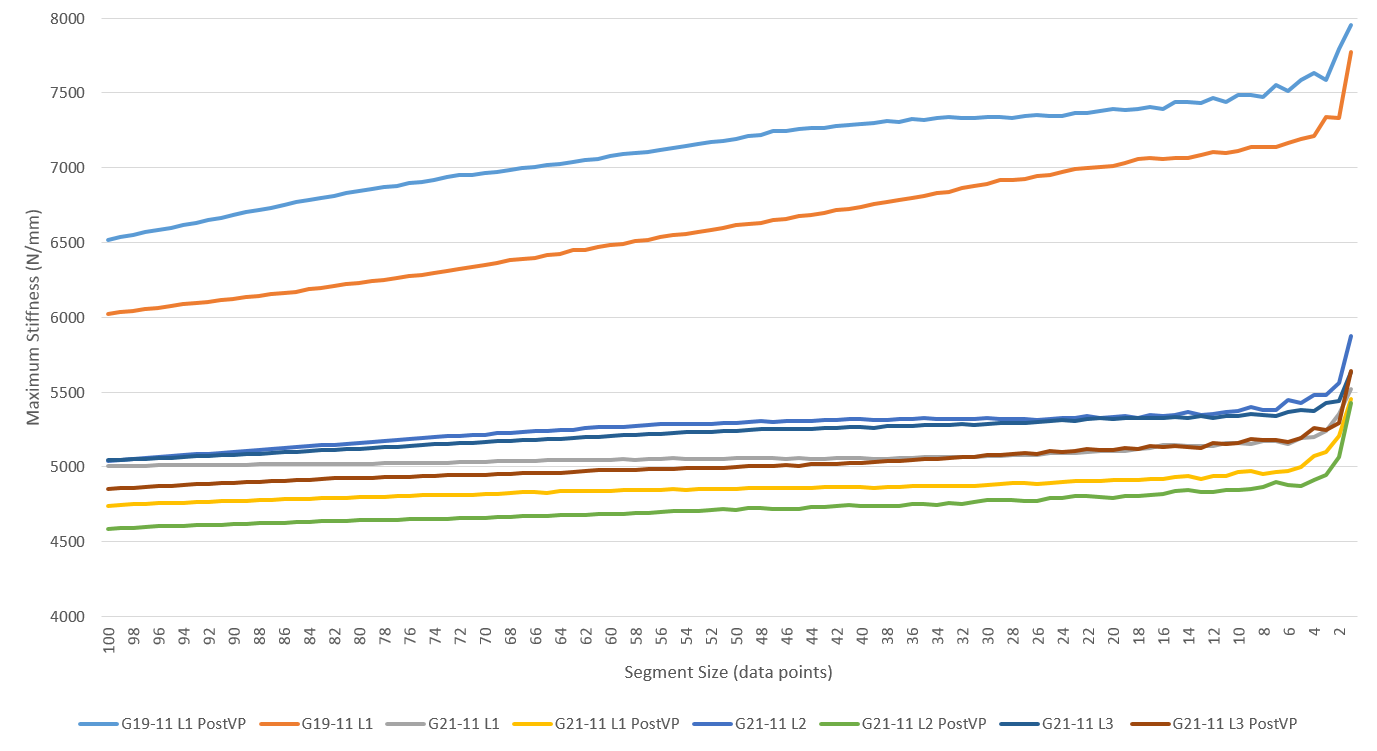
\includegraphics[width=6in]{Chapters/Chapter_HT_images/findStiffness_1incr.png}
  \caption{The effect of reducing the segment size on the maximum stiffness
    reported from four human vertebrae loaded to 2000 N pre and post
    augmentation. Using an increment size of 1 data point (0.0017 mm) and
    segment sizes of 100 to 1 data point (0.17 mm to 0.0017 mm).}
  \label{fig:findStiffness_1incr}
\end{figure}

\begin{figure}[ht!]
  \centering
  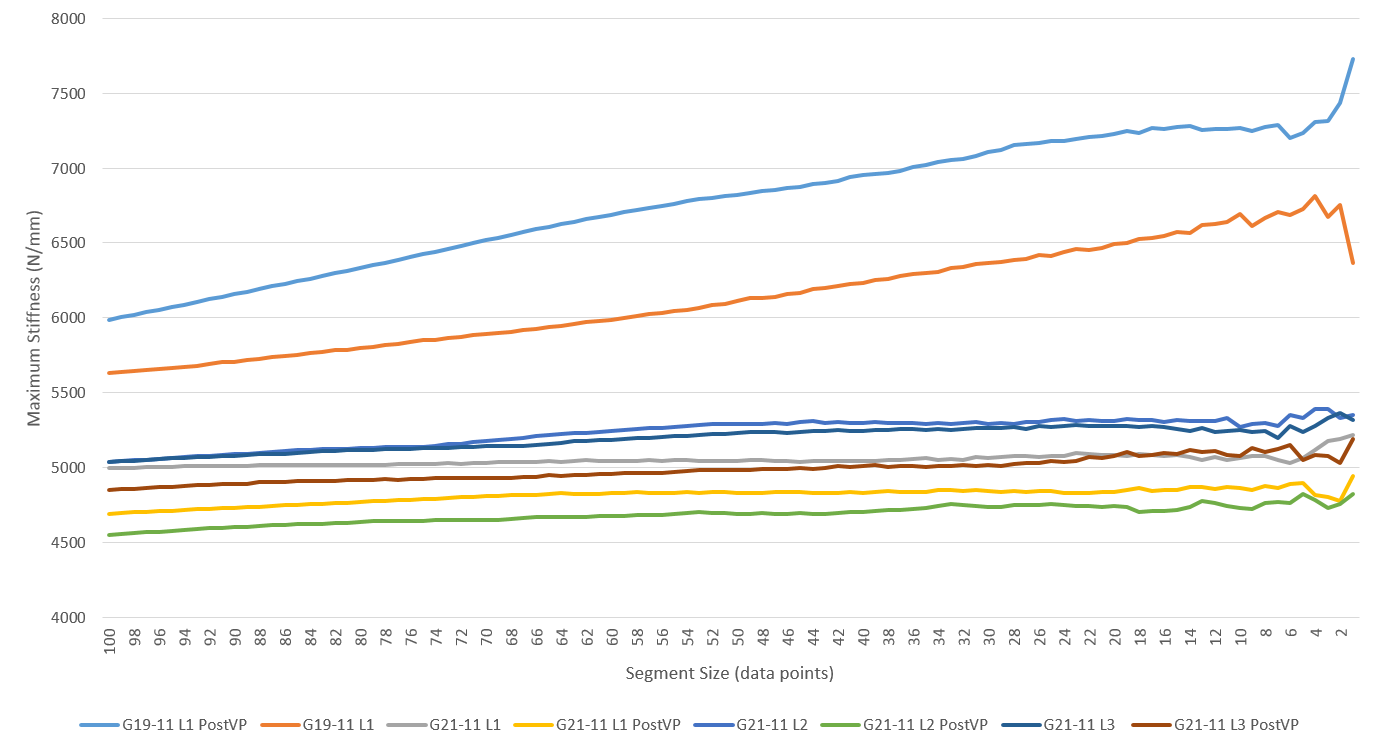
\includegraphics[width=6in]{Chapters/Chapter_HT_images/findStiffness_20incr.png}
  \caption{The effect of reducing the segment size on the maximum stiffness
    reported from four human vertebrae loaded to 2000 N pre and post
    augmentation. Using an increment size of 20 data points (0.0037 mm) and
    segment sizes of 100 to 1 data point (0.17 mm to 0.0017 mm).}
  \label{fig:findStiffness_20incr}
\end{figure}

Using an increment size of 1 data points width, as shown in Figure~\ref{fig:findStiffness_1incr} shows a smaller variation across the range of
segment sizes compared to using 20 points in Figure~\ref{fig:findStiffness_20incr}. The effect of both segment size and increment
size is especially evident for the two G19-11 L1 vertebrae both intact and post
augmentation where the stiffness continues to increase until the end of the test
at 2000 N. Meaning that there is a much smaller linear region for these two
specimens, hence requiring a smaller segment size to measure the largest
gradient.

Choosing values for the segment size to use moving forwards becomes difficult
given the large effect it can have on the measured maximum stiffness (a range of
over 1000 N/mm in the case the two G19-11 L1 tests). The segment size needs to
be small enough to capture the maximum stiffness while avoiding the noise when
using a segment size below 18 data points. Hence, a value of 20 data points was
chosen, a value that avoids the noise while being on the plateau of the lines.


\subsubsection{Repeated Loading}

Given the nature of the test (attempting to limit damage to the vertebrae)
especially during their initial intact load, the ability to derive errors
becomes difficult especially from a single load. To attempt to understand this
error four vertebrae having undergone augmentation were tested three more times
in an iterative fashion, removing each from the load testing machine, testing
the next specimen in the set and repeating. Removing the vertebrae from their
steel housing (instead of three tests while seated in the steel housing) allowed
the error in loading position and setup to be tested along with repeated loading
of the vertebrae to be tested.

The results of repeated loading can be seen in Figure~\ref{fig:exp_repeats}. All
four specimens show a reduced stiffness for the repeated loads following the
initial load, for which there are a few possible reasons. One possibility for
the reduction in stiffness is that it is a consequence of the freeze thaw cycle
that occurred between these tests. The second possibility is that the vertebrae
were still partially frozen while the testing took place. Finally, it could be
due to damage being caused during the initial load to 2000 N, shown in Figures~\ref{fig:G19-11_L1} to~\ref{fig:G21-11_L3} it is possible to see slight failure
in the three G21-11 vertebrae, although failure cannot be seen in the G19-11 L1
vertebrae. The frozen bar in Figure~\ref{fig:exp_repeats} shows how the
stiffness increases when the vertebrae are completely frozen, potentially
helping to explain the drop in stiffness found in the repeats. Further tests
will be carried out with three more repeats following another freeze thaw cycle
to attempt to answer this.

The iterative reduction in stiffness for the G21-11 L2 vertebrae can be
explained as damage being caused after each iteration. This can be seen in
Figure~\ref{fig:G21-11_L2}, with the three repeats each showing a yielding
before the 1600 N limit and a smaller maximum load and stiffness after each
repeat.

Figures~\ref{fig:G19-11_L1} through~\ref{fig:G21-11_L3} show the data for the
loading, from which the maximum stiffness values are found. This excludes the
initial cyclic loading, starts the loading at 50 N and displacement at 0 mm.

\begin{figure}[!h]
  \centering
  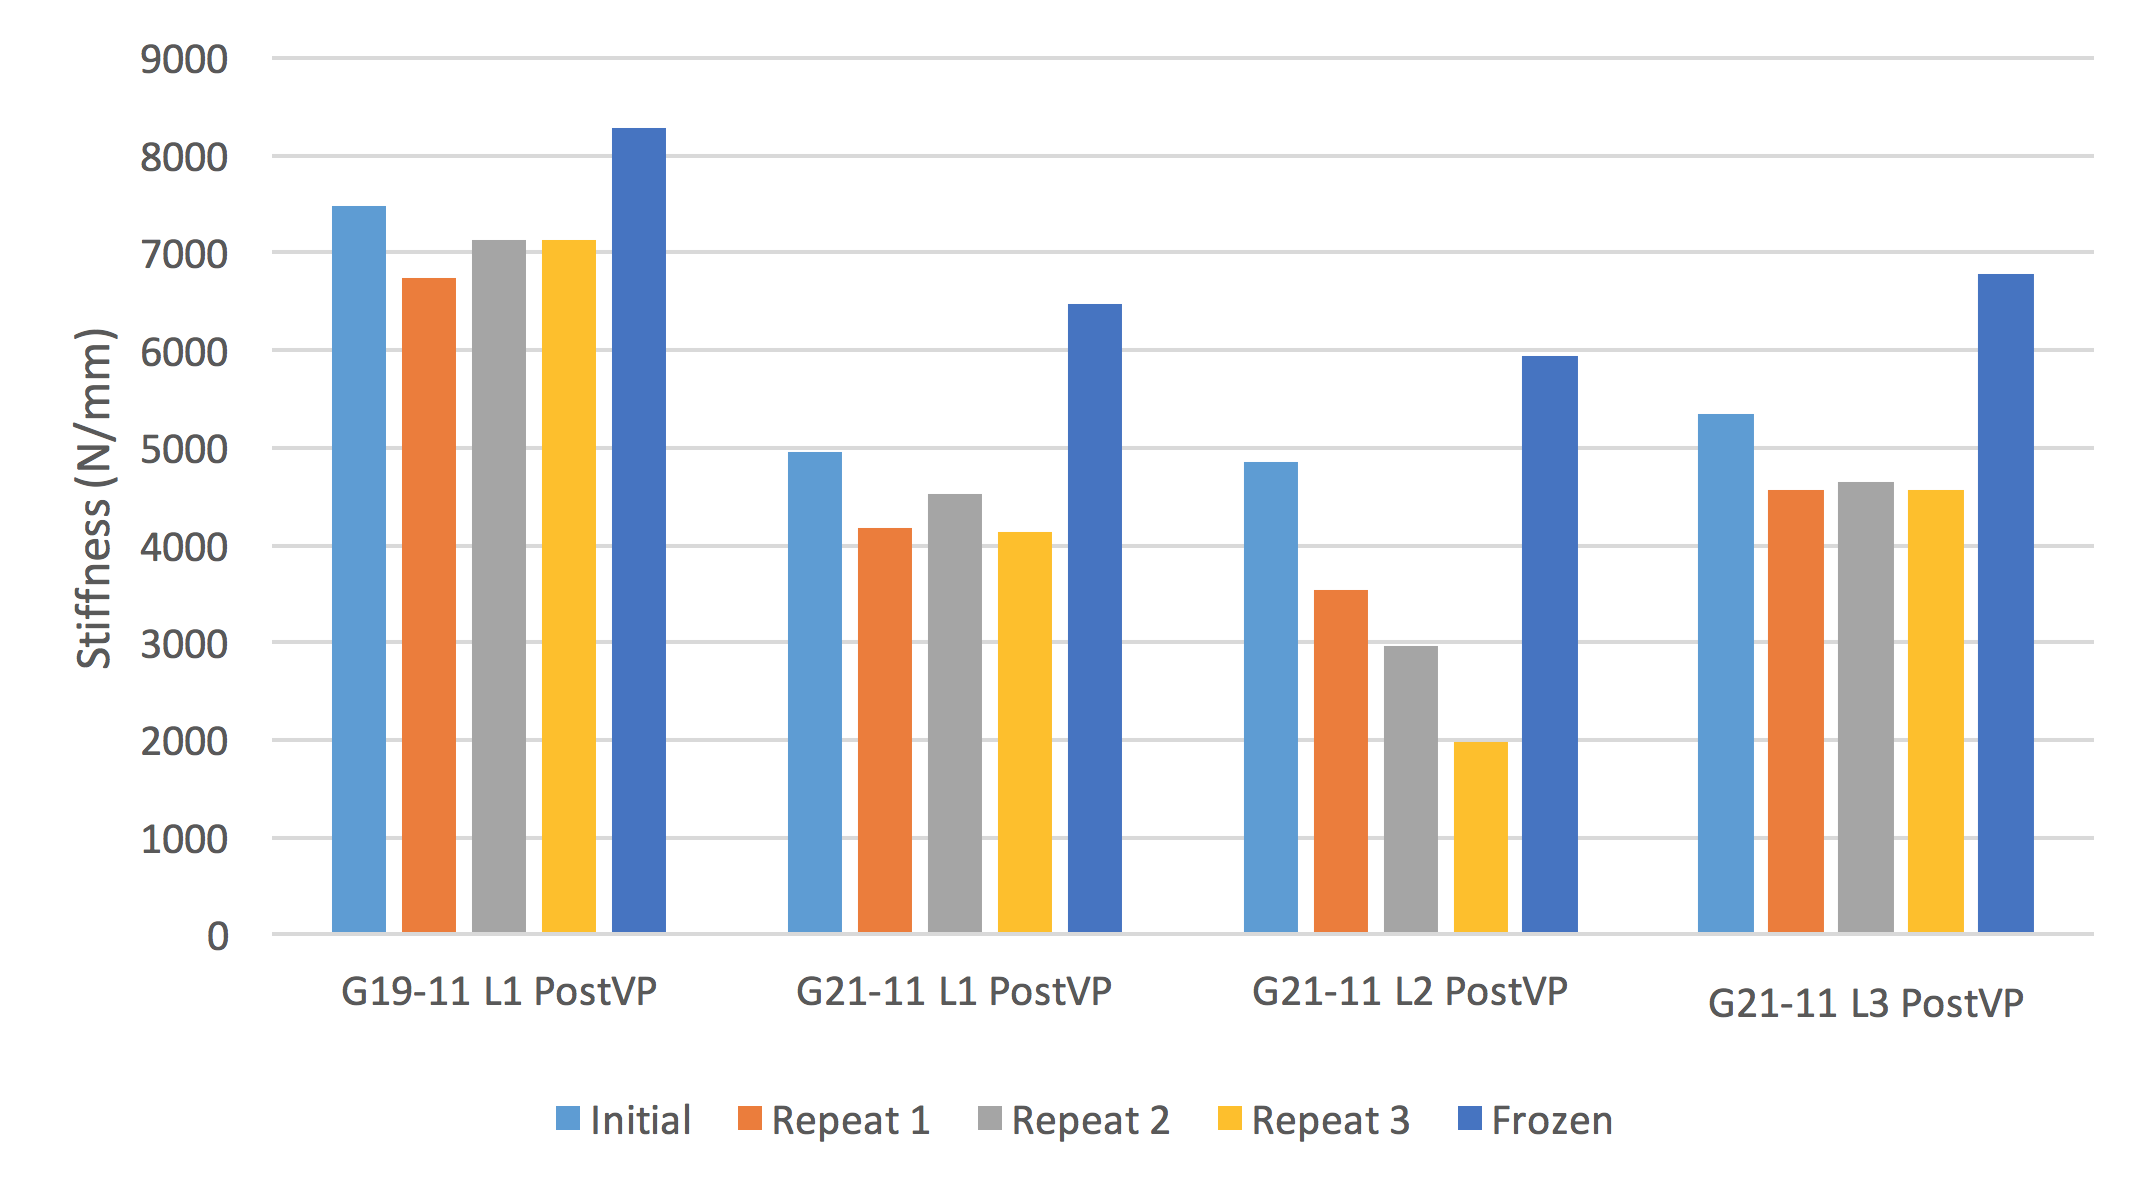
\includegraphics[width=6in]{Chapters/Chapter_HT_images/experimental_repeats.png}
  \caption{The stiffness of four augmented vertebral specimens over the course
    of an initial load, three repeated loads and a load while frozen. The intact
    specimen was loaded until 2000 N while the remaining four were loaded until
    1600 N.}
  \label{fig:exp_repeats}
\end{figure}


\begin{figure}[ht!]
  \centering
  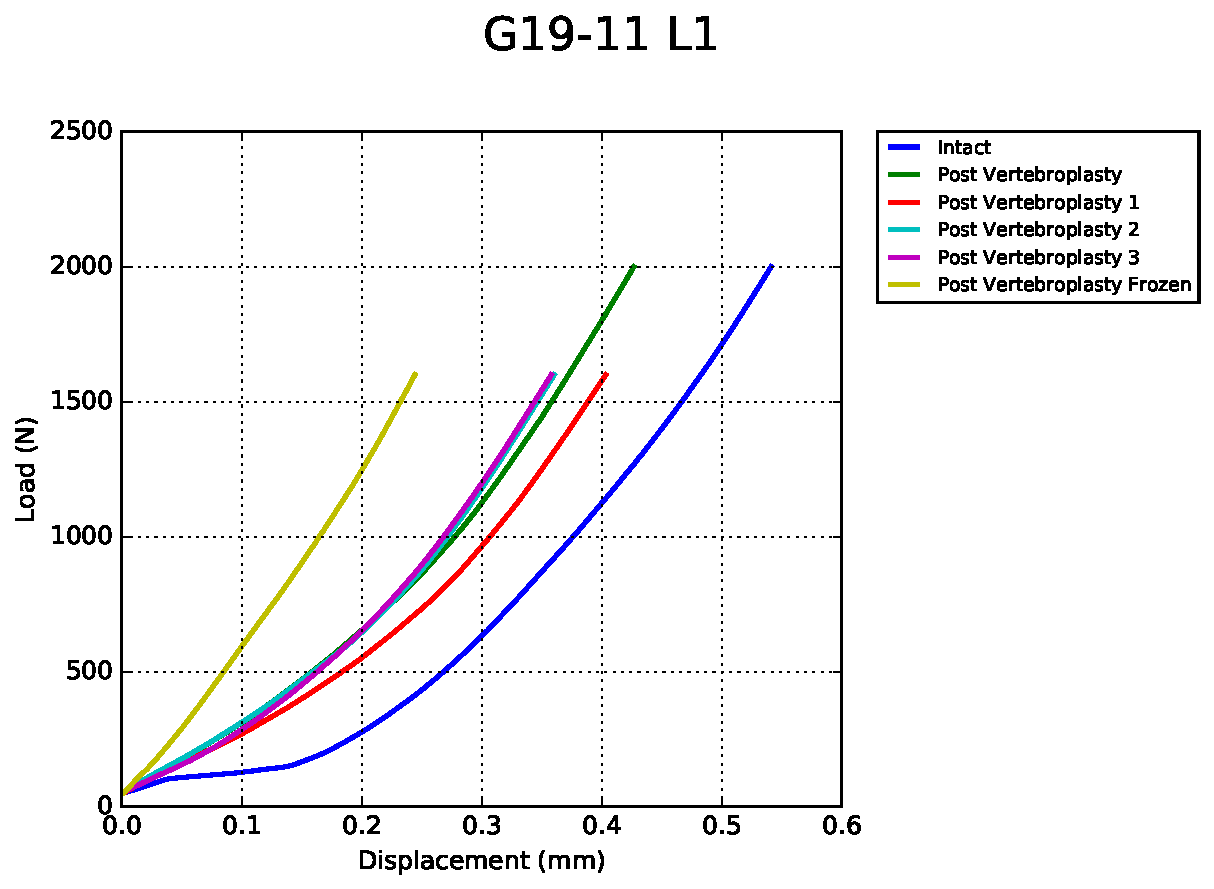
\includegraphics[width=4in]{Chapters/Chapter_HT_images/G19-11_L1.pdf}
  \caption{The load - displacement results for the G19-11 L1 vertebra. Showing
    results of the intact load and post augmentation load up to 2000 N and the
    repeats and frozen load up to 1600 N.}
  \label{fig:G19-11_L1}
\end{figure}

\begin{figure}[ht!]
  \centering
  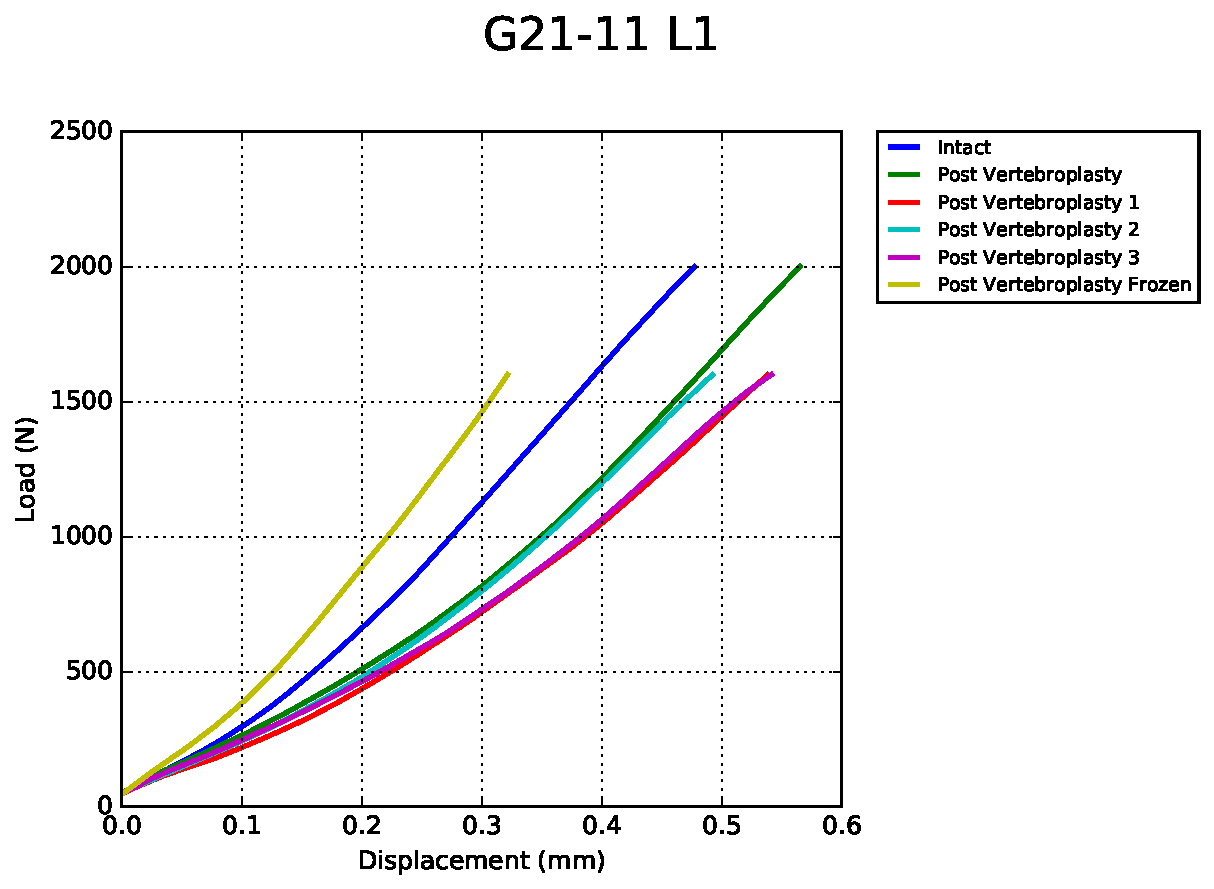
\includegraphics[width=4in]{Chapters/Chapter_HT_images/G21-11_L1.pdf}
  \caption{The load - displacement results for the G21-11 L1 vertebra. Showing
    results of the intact load and post augmentation load up to 2000 N and the
    repeats and frozen load up to 1600 N.}
  \label{fig:G21-11_L1}
\end{figure}

\begin{figure}[ht!]
  \centering
  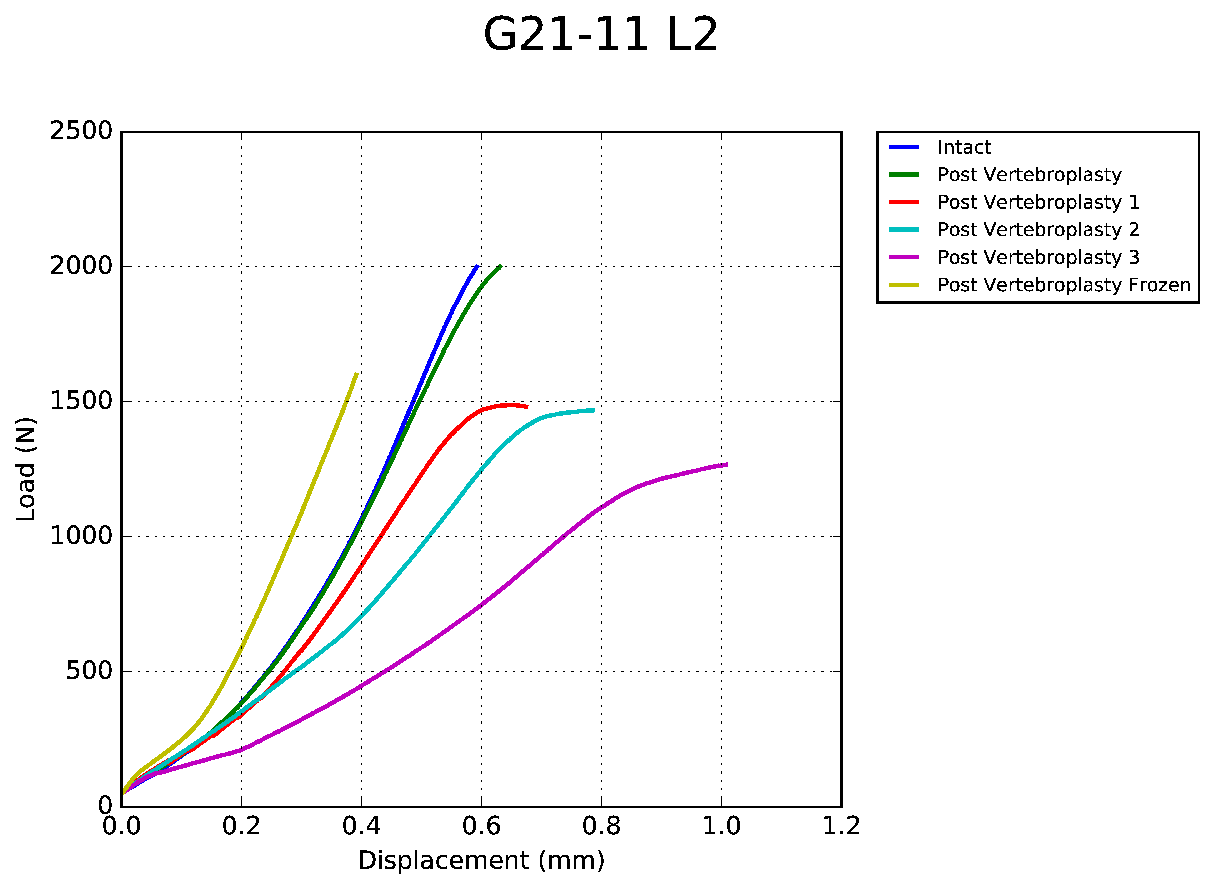
\includegraphics[width=4in]{Chapters/Chapter_HT_images/G21-11_L2.pdf}
  \caption{The load - displacement results for the G21-11 L2 vertebra. Showing
    results of the intact load and post augmentation load up to 2000 N and the
    repeats and frozen load up to 1600 N.}
  \label{fig:G21-11_L2}
\end{figure}

\begin{figure}[ht!]
  \centering
  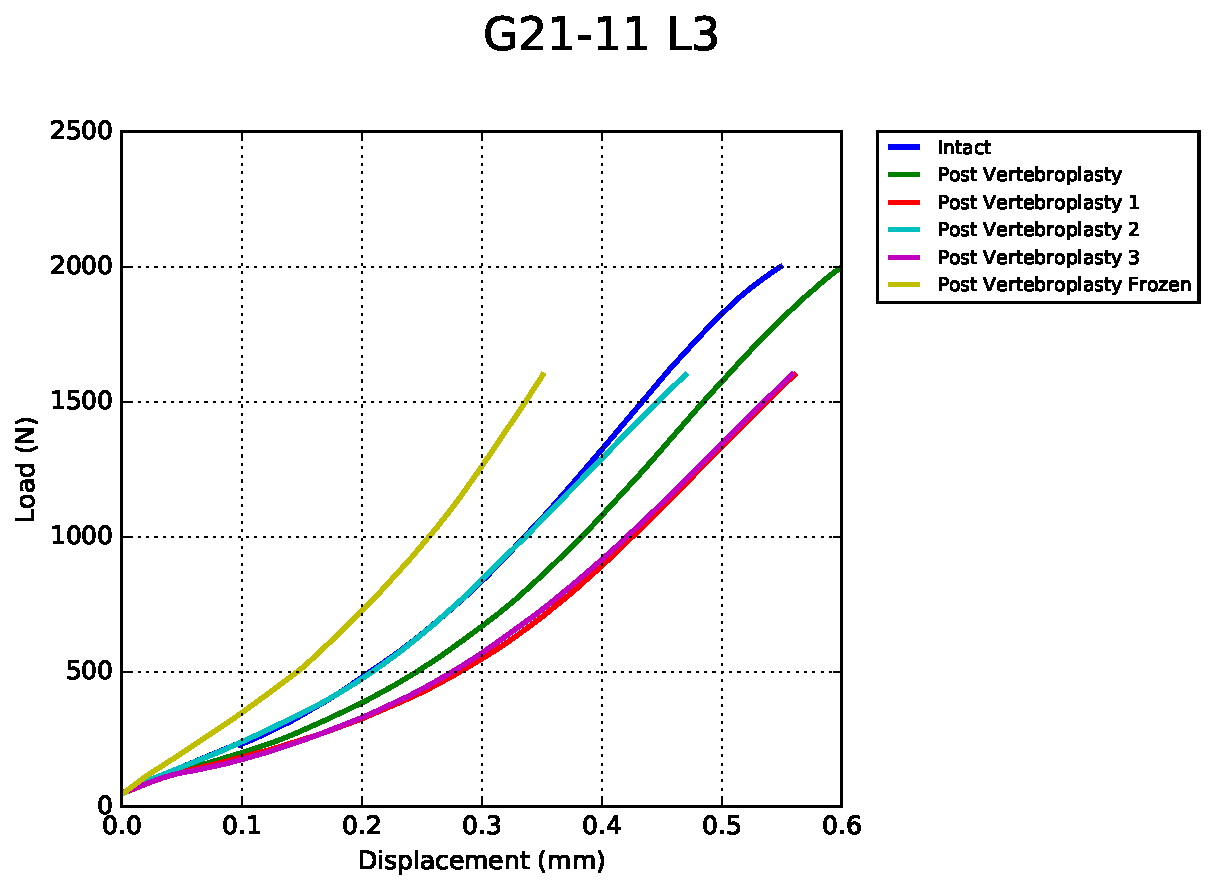
\includegraphics[width=4in]{Chapters/Chapter_HT_images/G21-11_L3.pdf}
  \caption{The load - displacement results for the G21-11 L3 vertebra. Showing
    results of the intact load and post augmentation load up to 2000 N and the
    repeats and frozen load up to 1600 N.}
  \label{fig:G21-11_L3}
\end{figure}






\subsection{Vertebroplasty}

Despite the development of methods for the augmentation of bovine tail
vertebrae, the methods for augmenting human vertebrae were altered due to the
different geometry and density. The human vertebrae, being much less dense, did
not require the vertebroplasty needle to be inserted with the aid of a mallet.
Instead the needle could be pushed by hand through the cortical shell and into
the vertebral body.

An additional difference was the approach with the needle, instead of entering
the vertebrae through their pedicles an oblique approach was adopted. This was
due to variation in pedicle diameter between the L1 - L5 lumbar levels and
therefore the potential to damage the region and its load sharing capabilities.
The oblique approach therefore avoided creating this damage to the pedicle-canal
region, especially for the vertebrae with narrower pedicles and instead created
much less damage to the vertebral body.

A final difference to the needle insertion methods was a change to the needle.
Here, a side opening needle was used, allowing the cement to be directed into
the anterior-centre region of the vertebral body as opposed to directly out of
the needle end.

An attempted 20 \% fill was used for the vertebrae, measuring the volume of the vertebral body from the $\mu$CT scans prior to augmentation.
However, despite stopping the injection upon cement leakage through vascular channels leading from the vertebral body surface inwards, cement loss occurred.
In addition to this, cement was also lost in the needle itself, where as the cement set the amount of cement remaining in the needle became difficult to measure.
This meant that the cement fill could not be measured though the amount of PMMA leaving the syringe due to leakage and needle losses.
Hence cement fill volume was measured using segmented $\mu$CT scans, the methodology of which is described below.

\subsection{Vertebrae Characteristics}

Identifying the different characteristics for the set of lumbar vertebrae has
importance in understanding trends and relationships between the experimental
and computational results. For example a larger degree of anisotropy and hence
more directionality aligned trabeculae would potentially give a more
experimentally stiff vertebra, despite otherwise similar characteristics. Given
that much of the vertebral characteristics depend on the trabecular structure it
is important to understand how this varies between specimens. Furthermore, any
calculations originating from a description of the trabecular structure require
a correct threshold to be applied to the $\mu$CT scan. This threshold describes
the limit of the trabecular bone and hence the start of either marrow or empty
space. To enable a fair comparison between vertebrae a region of interest was
selected from the vertebral body. Given the large variation in cortical shell
thickness, along with certain vertebrae containing large osteophytes and other
extra bone growth, the region of interest (ROI) was selected to be the largest
cylinder that could fit within the vertebral body while not capturing any of the
cortical shell.

\subsubsection{Histograms}

In order to understand the spread of brightness' from the set of lumbar the
histograms of the ROIs were plotted (Figure~\ref{fig:normalisedhistogram}).

\begin{figure}[ht!]
  \centering
  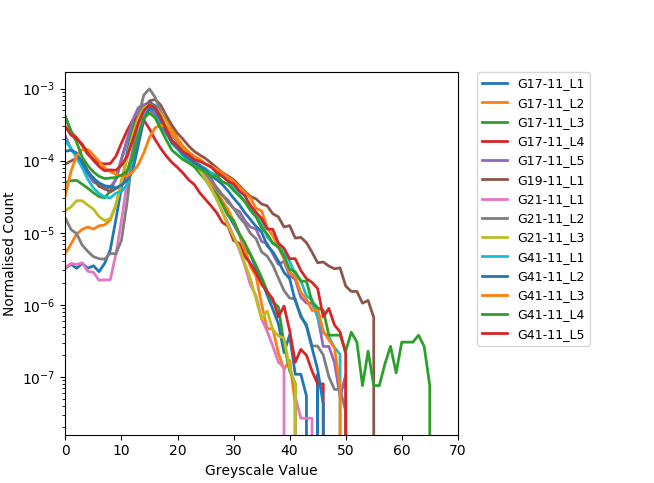
\includegraphics[width=4in]{Chapters/Chapter_HT_images/Normalised_Histogram.png}
  \caption{The normalised (with respect to the volume of the ROI) histogram data
    for the 14 lumbar vertebrae.}
  \label{fig:normalisedhistogram}
\end{figure}

The lower greyscale values represent the empty space within the ROI which
translates to regions where the bone marrow has exited the region, most likely
during the freeze thaw cycles. The peak in the histogram at an approximate
greyscale value of 16 is due to the bone marrow. The remaining portion of the
histogram represents bone, where variation is due to the differences in the
mineral content of the bone, with more mineralised bone appearing brighter on
$\mu$CT scans. The specimens ROIs that contain the brighter values are those
that contain osteophytes that contain more dense bone than the other cortical
shell, for example G19-11 L1.

\subsubsection{Threshold Optimisation}\label{th_opt}


The full resolution scan is imported into imageJ where the threshold optimisation is carried out.
The BoneJ plugin for imageJ is used for all of the trabecular structure metrics, with the optimise threshold tool being the focus here.
This tool is run on the region of interest using the default settings for the connectivity options seen in Table~\ref{tab:bonej}.
This chooses a threshold based on the peak in a connectivity against threshold plot and reports that value.
These values can be seen in Table~\ref{tab:optTH}, showing considerable across the range of vertebrae.
However, the differences in these suggested thresholds can grouped with the spine, for example: the G17 spine has a range between 15 to 17, while the G41 spine has an range between 18 to 20.
This promotes the idea that these differences are due to the bone mineralisation of the bone, especially given that the G17 spine is from a Female and G41 from a male.

However, given that the chosen value for the threshold will directly impact the reported metrics, a consistent value was chosen of 18. Using lower or higher values for the threshold usually results in the trabeculae being described as thicker or thinner respectively.
Hence, the difference in the mineralisation between specimens will still be captured when using a fixed threshold, given that the binary image will be down sampled before material properties are acquired.
The results in Table~\ref{tab:bv_tv_anis} show the BV / TV data and degree of anisotropy values for the 14 specimens using the fixed threshold of 18.
Similar trends to what could be seen from the optimise threshold results can be seen in the BV/TV data, with grouping between the
spines evident.
The G17-11 spine has a much lower bone volume fraction compared to the other spines, which suggests a more osteoporotic spine, most likely resulting in less stiff vertebra.

\begin{table}[ht!]
	\caption{Settings used for the ImageJ plugin, BoneJ: Optimise Threshold.}
	\label{tab:bonej}
	\centering
	\begin{tabular}{c|c}
    Options & Values \\
    \hline
    \hline
    Tests & 11  \\
    Range & 0.2 \\
    Subvolume Size & 256 \\
    Erosian Cycles & 0 \\
    Dilation Cycles & 0 \\
    \hline
	\end{tabular}
\end{table}

\begin{table}[ht!]
	\caption{The suggested threshold from the optimise threshold BoneJ tool for the 14 lumbar vertebrae in the set.}
	\label{tab:optTH}
	\centering
	\begin{tabular}{c|c}
    Specimen    & Suggested Threshold   \\ \hline \hline
    G17-11\_L1 & 17 \\
    G17-11\_L2 & 16\\
    G17-11\_L3 & 16\\
    G17-11\_L4 & 15\\
    G17-11\_L5 & 16\\
    G19-11\_L1 & 23\\
    G21-11\_L1 & 18\\
    G21-11\_L2 & 19\\
    G21-11\_L3 & 19\\
    G41-11\_L1 & 20\\
    G41-11\_L2 & 19\\
    G41-11\_L3 & 18\\
    G41-11\_L4 & 19\\
    G41-11\_L5 & 18\\
    \hline
	\end{tabular}
\end{table}

\begin{table}[ht!]
	\caption{BV/TV and degree of anisotropy (DA) values found using the ImageJ
    plugin BoneJ tools Volume Fraction and Annisotropy respectively using a
    threshold of 18.}
	\label{tab:bv_tv_anis}
	\centering
	\begin{tabular}{c|c|c}
    Specimen                       & BV/TV & DA\\ \hline \hline
    G17-11\_L1  & 0.174 & 0.387 \\
    G17-11\_L2  & 0.17  & 0.364\\
    G17-11\_L3  & 0.137 & 0.359\\
    G17-11\_L4  & 0.127 & 0.418\\
    G17-11\_L5  & 0.187 & 0.341\\
    G19-11\_L1  & 0.391 & 0.199\\
    G21-11\_L1  & 0.255 & 0.327\\
    G21-11\_L2  & 0.267 & 0.231\\
    G21-11\_L3  & 0.281 & 0.301\\
    G41-11\_L1  & 0.257 & 0.239\\
    G41-11\_L2  & 0.241 & 0.338\\
    G41-11\_L3  & 0.244 & 0.348\\
    G41-11\_L4  & 0.247 & 0.371\\
    G41-11\_L5  & 0.249 & 0.186\\
    \hline
	\end{tabular}
\end{table}


\section{Computational Methods}

The split between different modelling methods, computational and experimental is not terribly clear, given that computational methods are employed in the scanning and material property analysis described above.
However, the methods described in this section describe the process used to model non-augmented and augmented vertebrae, with associated sensitivity tests to understand the most appropriate approach to various aspects of the modelling process.

\subsection{Intact Vertebrae Modelling Sensitivity Tests}

Given the aims of the project - to include the models generated here into a
larger set of vertebral models for use in statistical shape modelling, it is
useful to model the vertebrae in a scanner independent method. A method for
doing this (BV/TV modelling method) uses a full resolution scan with the bone
regions segmented using a threshold. This full resolution segmented scan is then
downsampled to voxels with edge length of 1 mm, meaning that each voxel has a
greyscale value proportional to the BV/TV value for the region captured by that
voxel. Areas that contain more bone will therefore have a higher greyscale
value. This method is purely dependant on the threshold selected defining the
bone and hence, given that threshold values can be repeatedly and correctly
selected with the methods shown in Section~\ref{th_opt}, it is scanner independent.

Other sensitivity studies present difficulties due to the models reliance on the underlying greyscale background.
This is due to the greyscale optimisation process required to obtain a new conversion factor between the greyscale values and the Young's modulus for every change made to the material properties or boundary conditions of the models.
This is in order to understand the effect the change has on the agreement between experimental and computational results, and because a change to the material properties or boundary conditions may not have a systematic or uniform effect on the results.
Due to this, simple sensitivity tests become difficult, including common convergence studies.

\subsubsection{BV/TV Modelling Method}\label{bvtv_method}

This method gives the opportunity to keep much of the detail that is often lost when downsampling image data.
Specifically, the method described gives the vertebral models much more definition of the cortical shell and internal trabecular structure while maintaining the 1 mm cubed resolution and the computational cost benefits associated with that.
The method follows that found in a study by Robson Brown et al.
\cite{RobsonBrown2014} with a few minor changes. The scans are converted from the ScanCo proprietary ISQ format into a stack of TIFF files using an in house Matlab script, which in additionally reduces reduces the 16 bit data to 8 bit images.

The set of vertebral specimens were split at this stage into two sets, allowing
an understanding of how the bone volume fraction method affects the results compared to the method described in Section~\ref{finite-element-modelling-methods}.
To the set using the bone volume fraction method a threshold was applied at the full 82 $\mu$m resolution.
This threshold was chosen to be a greyscale value of 18, the mean of the values described in section Section~\ref{th_opt} and was applied to the scan stacks in imageJ.
Once the binary stack was created a Gaussian filter was applied, also within imageJ, with $
\sigma_{x,y,z} = 1 $.
This was applied in order to remove speckling found surrounding the end-caps and some of the other noise visible in the scans.
The two stacks of images are then imported into ScanIP; carried
out by opening one stack of images (the original stack) and then importing a
second background (the binary image stack). Both backgrounds are downsampled to
voxel sizes of 1 mm$^3$, with the (originally) binary stack being used to create
the mask for the vertebrae and the original stack being used for the end-caps.
Greyscale material properties for the vertebral mask are taken from the binary
stack, while the remainder of the methods follow the same process as the
original method.

%\begin{figure}[ht!]
%  \centering
%  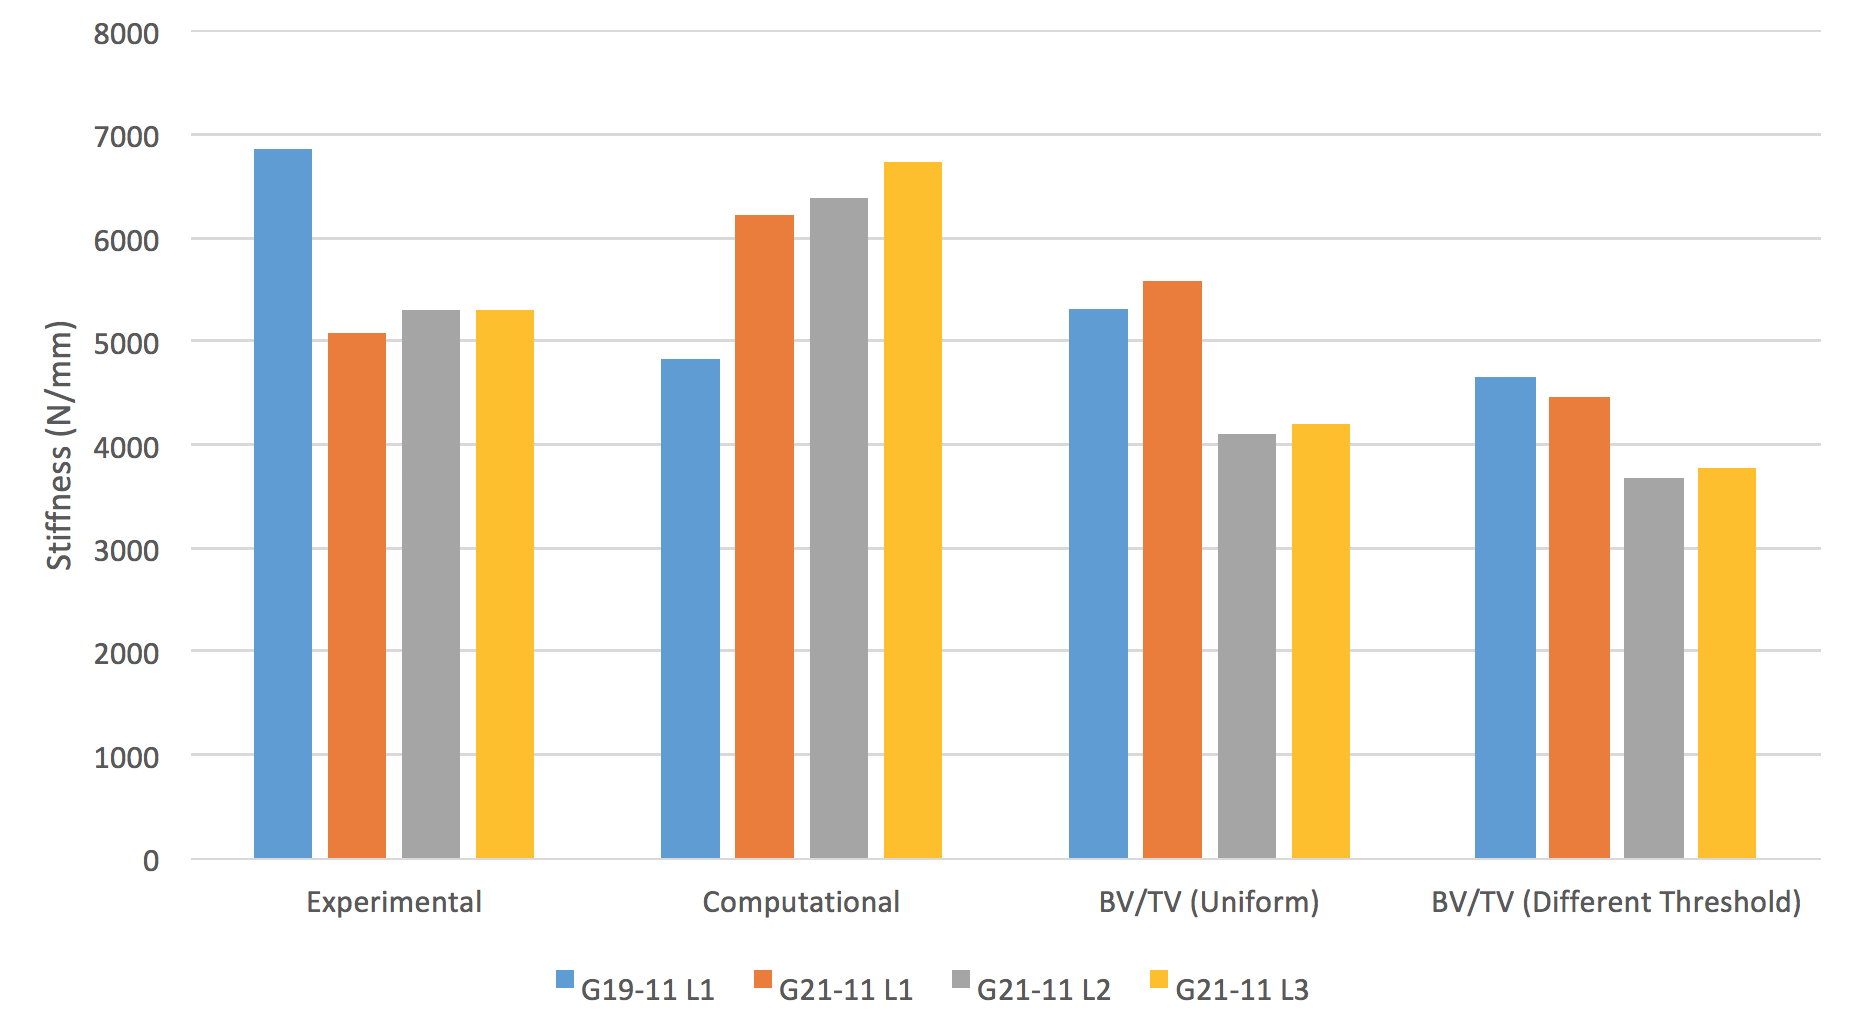
\includegraphics[width=6in]{Chapters/Chapter_HT_images/diffModellingMethods.png}
%  \caption{The stiffness results of three different FE methods for four intact
%    human vertebrae compared to the experimental stiffness results. Interest
%    should be drawn to the ratio between specimen models rather than the values
%    themselves, given that the conversion factors between greyscale values and
%    Young's modulus have not been optimised at this stage. Results show the
%    difference between the currently used method of modelling the vertebrae and
%    the BV/TV based methods (both with uniform thresholds and different
%    thresholds for each specimen).}
%  \label{fig:diffModellingMethods}
%\end{figure}




%\subsubsection{Predicting Vertebral Yield Point}\label{predYield}

\subsubsection{Load Position Sensitivity}

In order to understand how the vertebrae respond to different loading positions, eight different positions were tested, shown in Figure~\ref{fig:loading_pos}. The same boundary conditions, along with the 1 mm of displacement described above were applied to the different loading positions and the change in stiffness was recorded.

\begin{figure}[ht!]
\centering
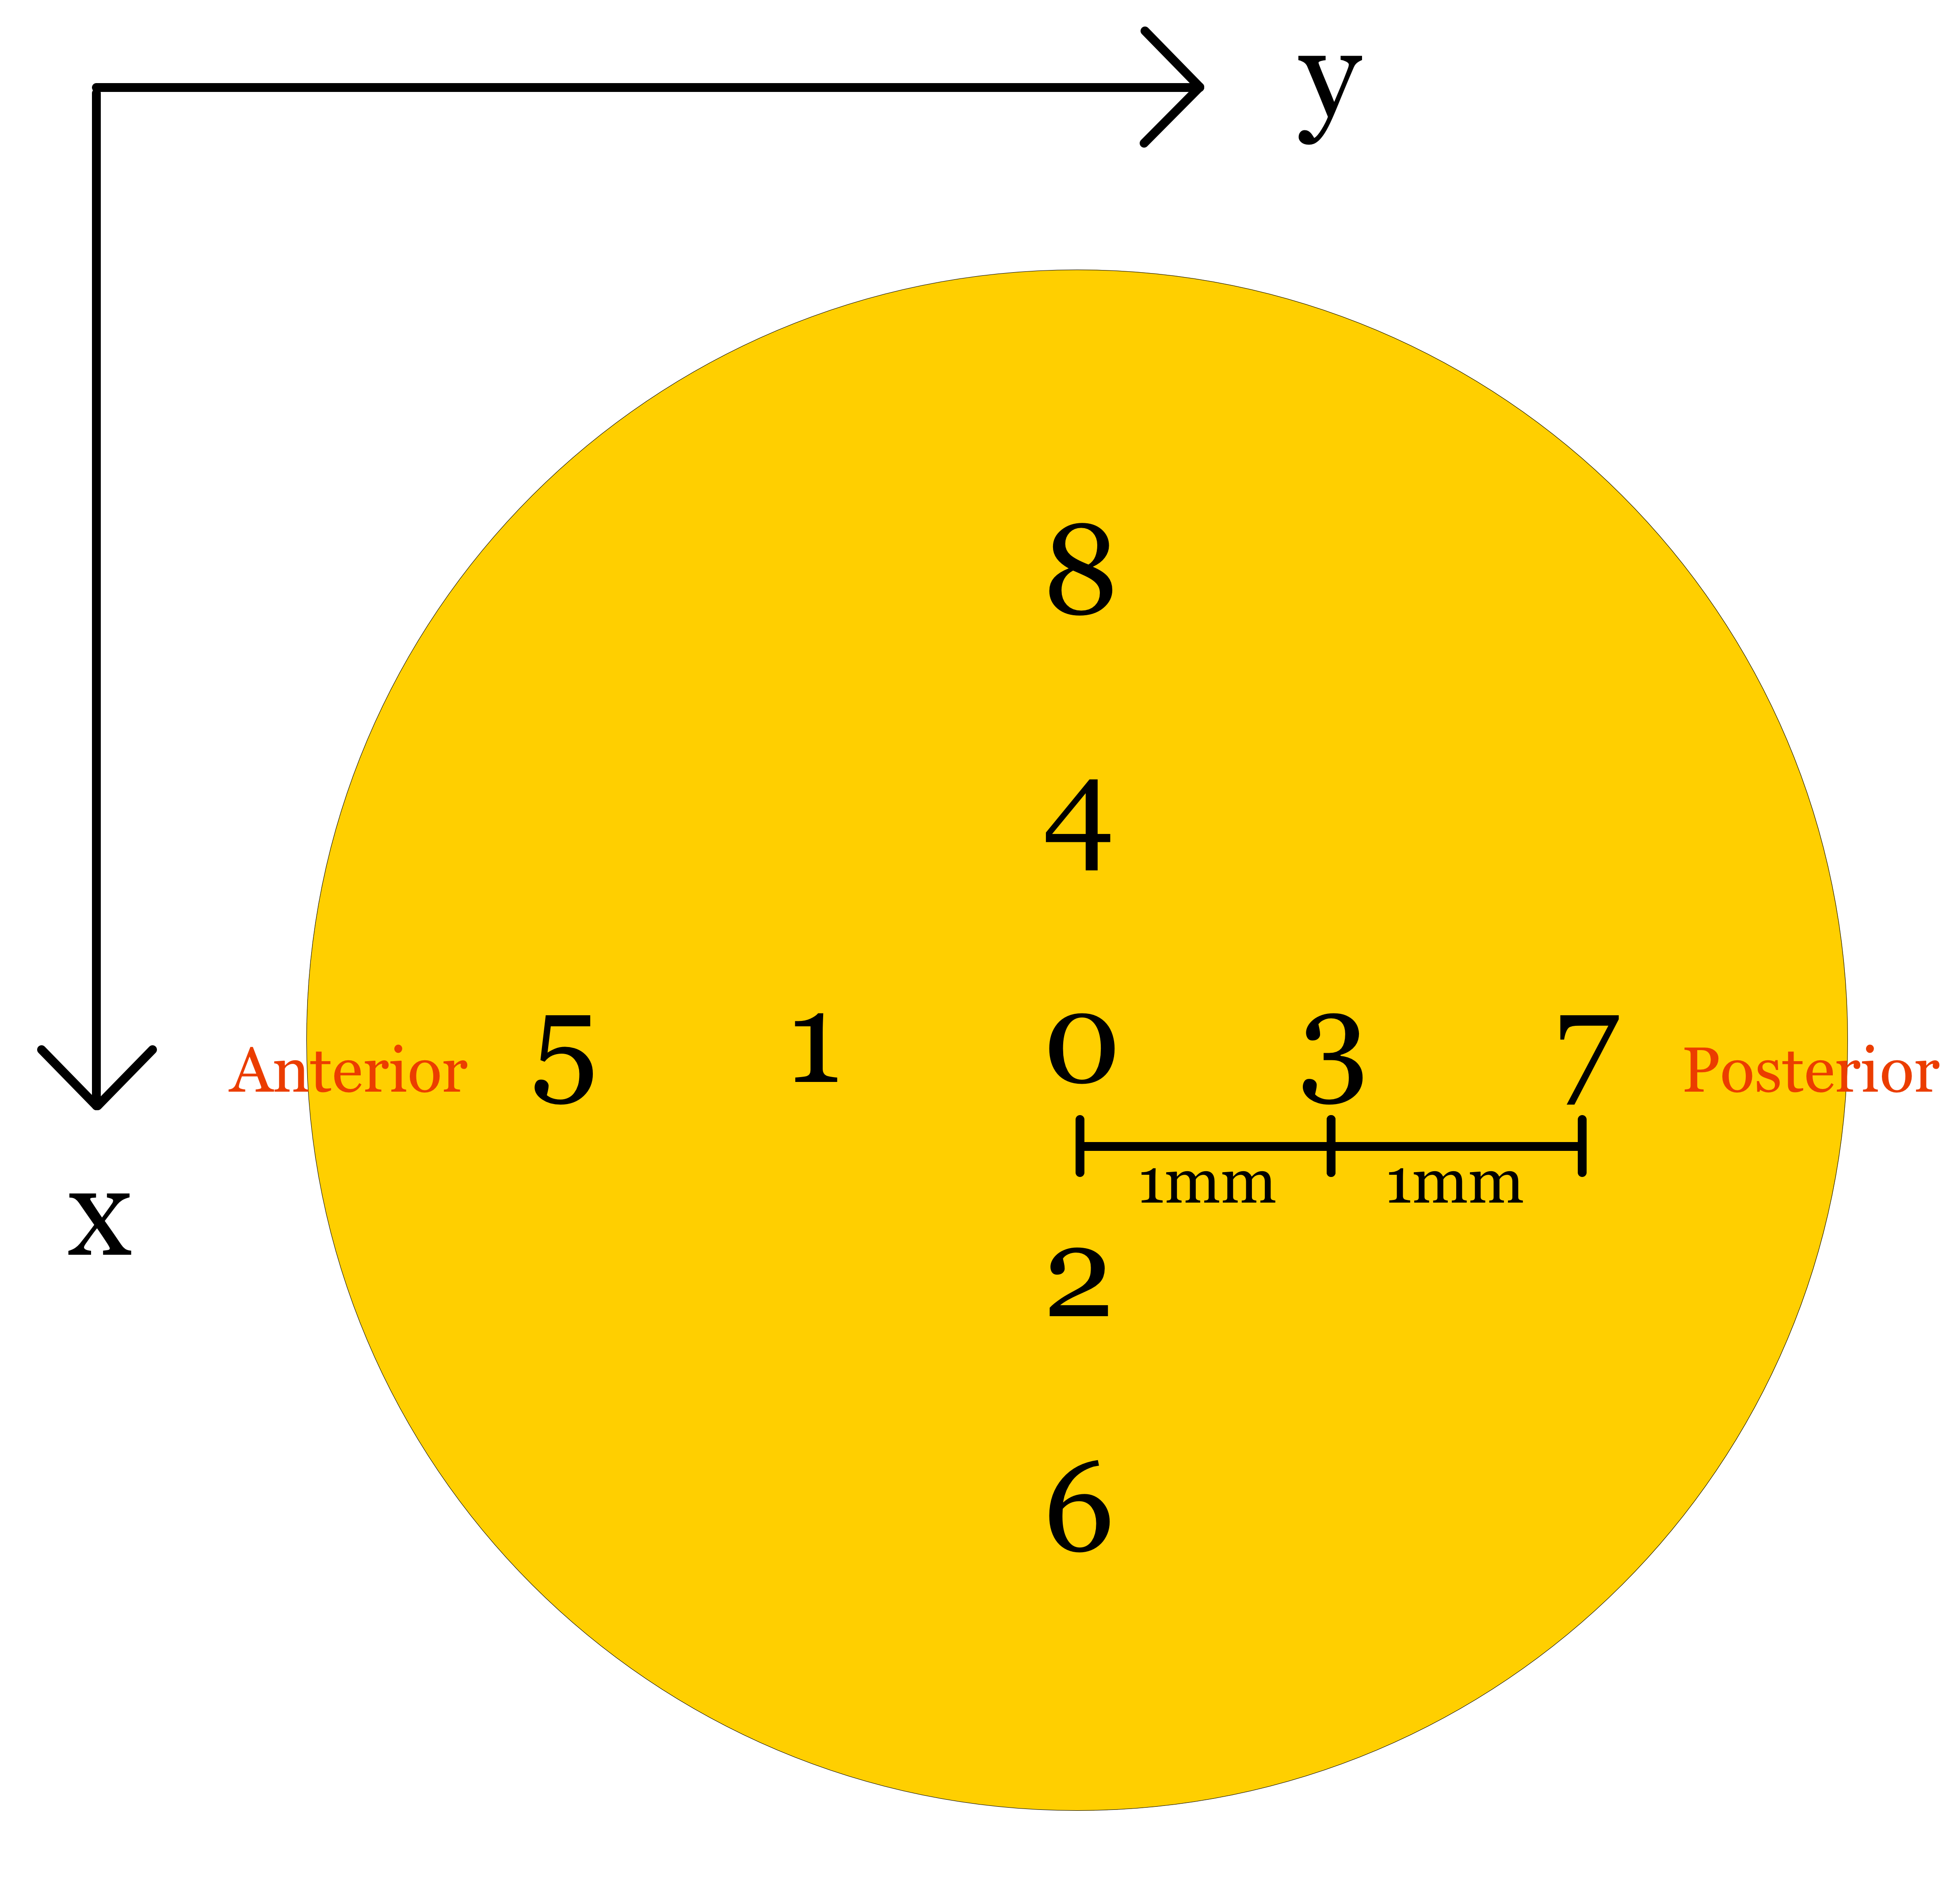
\includegraphics[width=6cm]{Chapters/Chapter_HT_images/Loading_positions.png}
\caption{The loading positions used for the load variation tests. Position 0 is the original, central loading position, with 1 - 4 being 1 mm away from the centre and 5 - 8 being 2 mm away from the centre.}
\label{fig:loading_pos}
\end{figure}


The results of the load position sensitivity tests (Figure~\ref{fig:hum_load}) show that more posterior loads (above denser bone) result in higher stiffness's while anterior loads result in a reduced stiffness. Loads lateral to the central loading point resulted in smaller reductions in the stiffness of models.

It also shows that the effect of movements of 1 mm away from the experimental loading position only changes the stiffness by approximately 5 \%.
Given the resolution of the models is limited to 1 mm, the accuracy of the selection of the experimental loading positions is also limited to 1 mm.
The maximum 5 \% change to the stiffness when posterior or anterior may describe some of the error seen when comparing the experimental and computational results.

\begin{figure}[ht!]
\centering
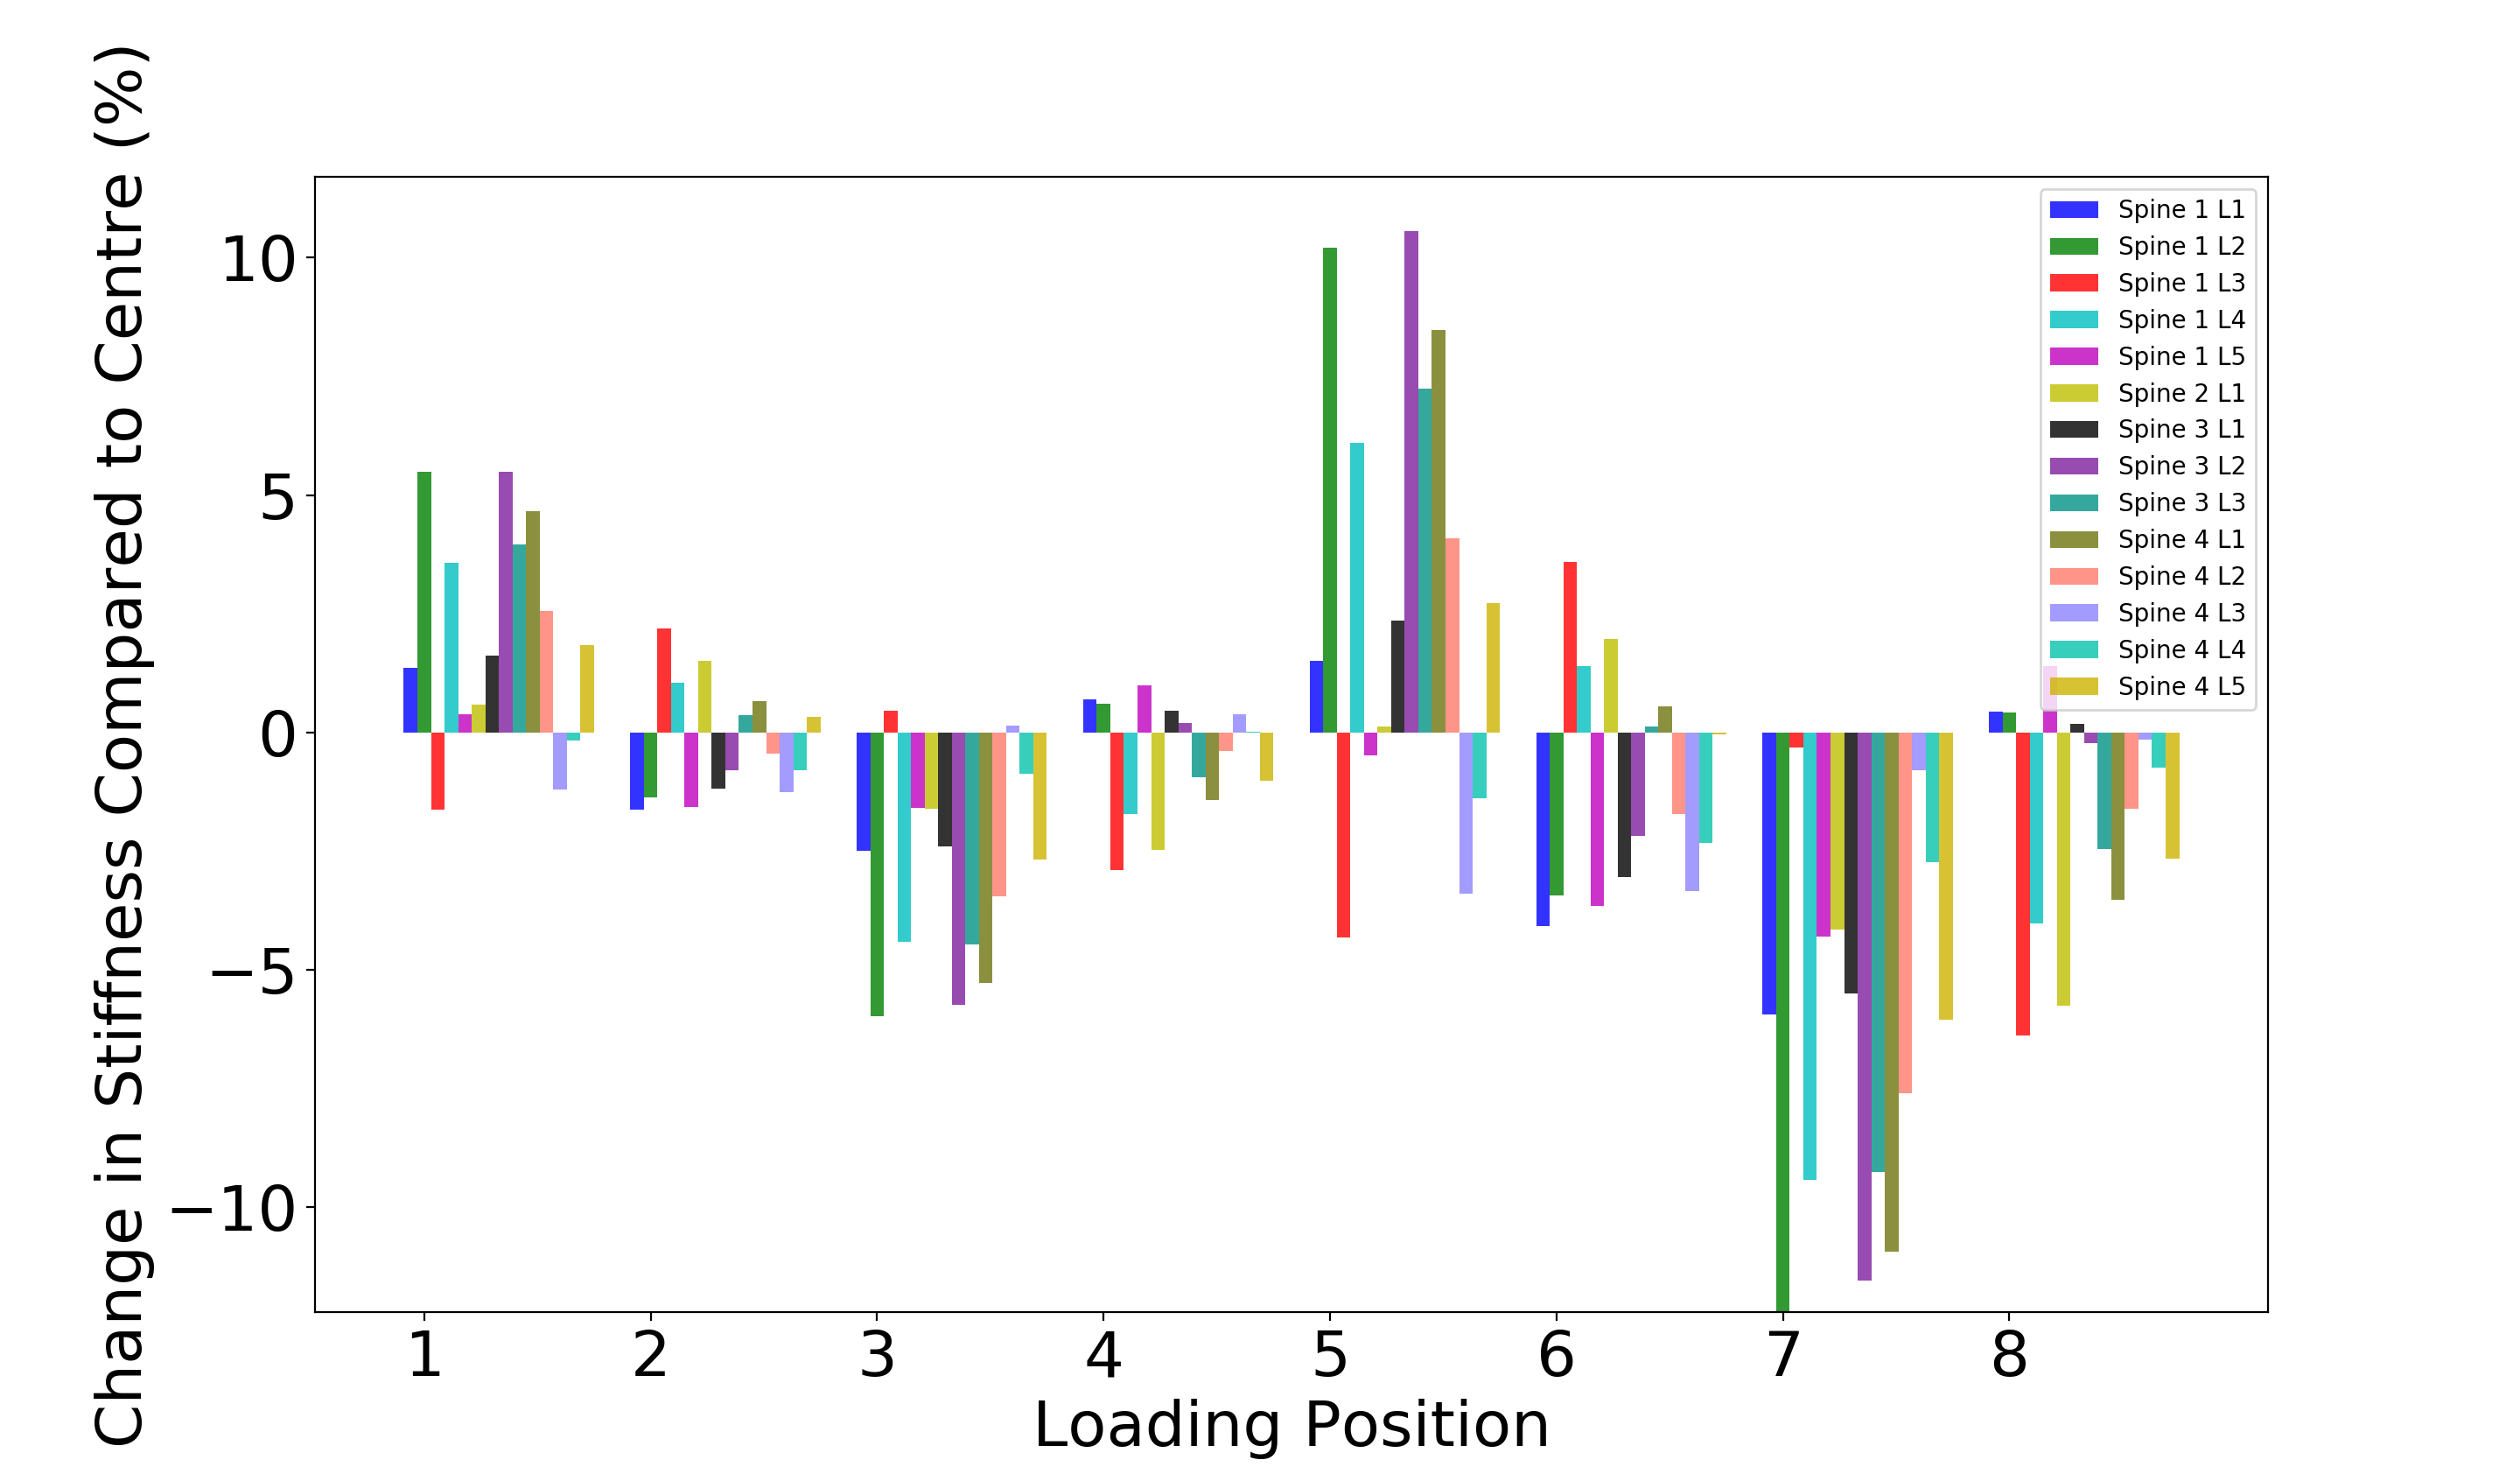
\includegraphics[width=\textwidth]{Chapters/Chapter_HT_images/human_fossil_loading.png}
\caption{The effect of the loading position for the human lumbar vertebrae, shown as a percentage change compared to a central loading position.}
\label{fig:hum_load}
\end{figure}



\subsubsection{End-cap Depth \& Contact sensitivity}

The stress distribution at the surface of the vertebral body shows high stress at the edges of the cement endcaps, at both the top and bottom of these regions.
Experimentally the endcaps are merely moulded to the shape of the top and bottom of the vertebral body, however, previous work and other studies have used tied contact between the bone and endcaps, removing any motion between the two and locking neighbouring nodes together.
Additionally, the depth of these endcaps varies between 5 mm and 20 mm depending on the shape of the vertebral endplates.
The more concave the vertebral endcap was the more cement was required to fill the space forming a flat cement surface.

Given this variation, tests identifying the effect of changing the endcap depth were carried out using FEA models with different depths of $\pm$ 1, $\pm$ 2 and $\pm$ 3 mm for the top and bottom endcaps independently and together.
Additionally, different interactions between the bone and cement endcaps were tested.
This included the current standard method of a tied interaction and replacing this with a frictionless contact between the two materials.
Finally, the effect of changing the cement endcap depth with the frictionless contact was also investigated, along with variations to the properties of the frictionless contacts.
This was carried out given that, experimentally, there is no tied contact between the PMMA and the bone due to the lack of adhesive properties for the PMMA.

The endcap depth was altered by adding and removing layers within the model file in ScanIP, re-meshing the model and running the files using the same Abaqus python scripts.
Endcap contacts were changed within the Abaqus python scripts, by firstly removing the ties between the endcap and the vertebra.
An interaction property was created with tangential behaviour set to frictionless and normal behavior with properties: $pressureOverclosure=HARD,  constraintEnforcementMethod=Default$ and the final option was experimented with, $allowSeperation=ON/OFF$.
The $allowSeperation$ variable determines whether separation is permitted once contact is established and models ran correctly with it set to its default of $ON$.
However, when experimenting with the effect of loading position, especially with loads applied far from the vertebral centre, the solver struggled to converge.
Disallowing separation after contact was shown to have a small effect on the results (the outputted stiffness) and allowed the models to run to the completion of the job.
The remaining settings were set to the default for a generic contact: 
\begin{minted}{python}
	initialClearance=OMIT, 
	adjustMethod=None, 
	sliding=SMALL, 
	enforcement=NODE_TO_SURFACE, 
	thickness=ON, 
	supplementaryContact=SELECTIVE, 
	interactionProperty=contactName, 
	smooth=0.2, 
	bondingSet=None
\end{minted}

Further tuning of these variables to see if an improved agreement could be achieve would be a simple, though time consuming addition to this sensitivity test due to the greyscale conversion factor optimisation process required to test each option.

\subsection{Modelling Augmentation}

Given the limited validation of models achieved using bovine tail vertebrae (due to the reasons discussed in Section~\ref{bov:results}), a range of different material properties and approaches to modelling the bone-cement interface were investigated.
In addition to varying the material properties of the injected volumes of cement, the effect of using a combination of scans from before and after augmentation has been experimented with.
To achieve this scans of pre/post augmentation were registered.
This method utilised the BV/TV method described earlier, where the non-augmented full resolution thresholded scan is registered to the full resolution augmented scan.

\subsubsection{Registration of $\mu$CT Scans}

Artificial brightening of regions surrounding the internal cement (specifically the concentrated volumes of barium sulphate and the artefacts associated) affect the material properties that are applied to the material, seen in the right-hand image in Figure~\ref{fig:reg_demo}.
To bypass this effect the two models, intact and post-augmentation models can be registered - translating them into the same spacial location.
This allows the cement to be defined, masked and modelled based on the post-augmentation scan and the remaining vertebra to be defined from the intact scan, the same background used for the intact models.
While the shape of the vertebra may have been changed over the course of its two loads, this change is less than what can be seen at 1 mm resolution and is not apparent during the registration process carried out at 82 $\mu$m resolution.
Additionally regions that have experienced damage through the insertion of the needle, yet do not contain cement, will also be neglected using this method.
However, the same justification can be made, where this is unlikely to have any affect at 1 mm resolution.

Registration of the images was carried out in 3D Slicer, using scans of the segmented, full-resolution, non-augmented vertebrae and the full-resolution augmented vertebral scans.
The method of registration was a landmark based approach using three landmarks for each vertebra, translating the scan of the augmented vertebrae.
These points were selected at superior of one pedicle, the inferior of the other pedicle and the inferior anterior of the vertebral body.
The selection of these points proved to provide a repeatable registration of the vertebrae, without selecting superfluous landmarks.
Once registered the resulting translated augmented vertebrae scan was cropped with respect to the non-augmented scan to provide an aligned and registered pair of scans.

\begin{figure}[ht!]
  \centering
  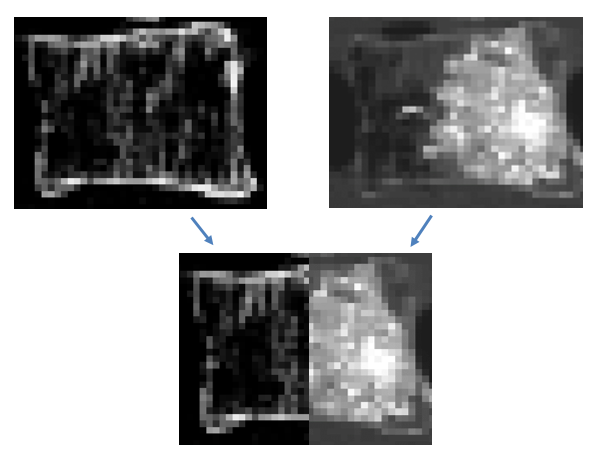
\includegraphics[width=4in]{Chapters/Chapter_HT_images/reg_demo.png}
  \caption{An illustration of the registration process, registering the non-augmented scan (left) with the augmented scan (right). The images are at 1 mm resolution, showing the artifacts created by the barium sulphate when viewed at this resolution, while to increase accuracy the registration carried out in Slicer 3D was at the full 82 $\mu$m resolution.}
  \label{fig:reg_demo}
\end{figure}

\subsubsection{Registered Scan Model Generation}

The augmented models using the registered scans were created in ScanIP, following similar methods to the bone volume fraction method described in Section~\ref{bvtv_method}.
The initial step was to import the registered augmented scans and apply an initial downsample to a resolution of 0.5 mm$^3$.
This resolution provided enough detail to capture the detail of the injected cement volume without increasing the computational difficulty and therefore time to segment the scans.

To segment the three regions (background, bone and endcaps, and injected cement) it was found that the most reproducible and accurate method was to use the Otsu thresholding process \cite{sezgin2004survey}, a filter that is built in to ScanIP\@.
It was used to find three masks in the scan and works on a threshold clustering method.
In this case searching for three clusters or masks separated by different thresholds and returning a mask that described the background, the bone and endcaps and the cement region.
From this only the cement mask was retained and underwent a flood fill filter, removing empty voxels found within the description of the mask.
The mask and background were then downsampled to 1 mm resolution and cropped to the same dimensions as the non-augmented model.
From the non-augmented model, the masked describing the vertebra, the endcaps and the background of the vertebra where imported.
The origin of the masks coming from the two backgrounds can be seen in Figure~\ref{fig:mask_demo}.

\begin{figure}[ht!]
  \centering
  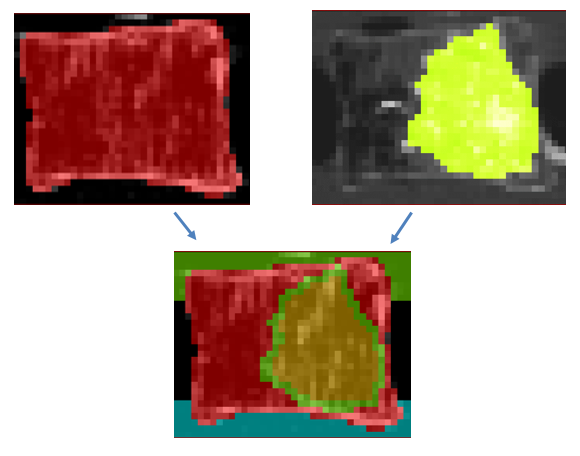
\includegraphics[width=4in]{Chapters/Chapter_HT_images/mask_demo.png}
  \caption{An illustration showing the origin of the masks from the non-augmented scan (left) and the augmented scan (right).}
  \label{fig:mask_demo}
\end{figure}


\subsection{Measuring the Vertebral Body \& Augmentation Volume}

While the volume of the vertebral mask can be measured directly within ScanIP or Abaqus, this volume includes the remainder of the pedicles.
The size of the pedicles that remain after their removal during dissection varies between level and spine and is especially different with the level five vertebra, where the shape and size varies dramatically.
To account for this variation and to get a more accurate cement fill percentage for the augmented models elliptic cylinders were fitted to the vertebral body as shown in figure~\ref{fig:cyl_fit}



\begin{figure}[ht!]
  \centering
  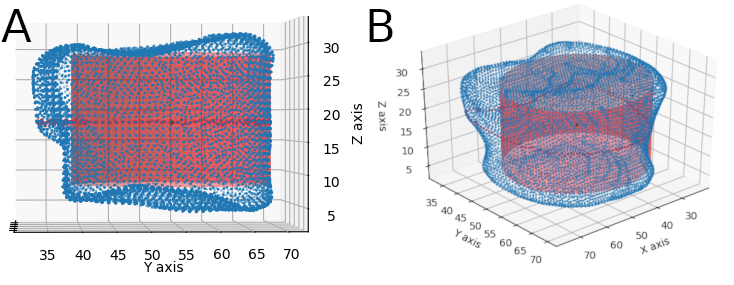
\includegraphics[width=5in]{Chapters/Chapter_HT_images/cyl_fit_ful_iso_both.png}
  \caption{A diagram showing the fitting of the cylinders to the vertebral body, where the point cloud describing the vertebra comes from an STL file, the red ring shows the points included in the mid-slice and the central red dot indicates the center of the mid-slice.}
  \label{fig:cyl_fit}
\end{figure}

Vertebrae that contained a vascular channel, seen in figure~\ref{fig:cyl_channel}, had the channel removed by filling the space in ScanIP.
This was carried out for two main reasons: the first was to allow accurate fitting of the cylinder into the vertebral (to avoid the problems shown in figure~\ref{fig:cyl_channel}) and to remove problems with the cement being exposed when modelling augmentation and the extra contacts / interfaces that are created.
Models with the vascular channel removed were compared to the original models and it was found that there was less than 0.5 \% difference for the set.
This was due to the elements used to fill the channel having material properties based on the greyscale, which had values of approximately zero, given the nature of the channel.
Due to the lack of any effect in removing the channel the vertebra models of augmentation did not include the vascular channel.

\begin{figure}[ht!]
  \centering
  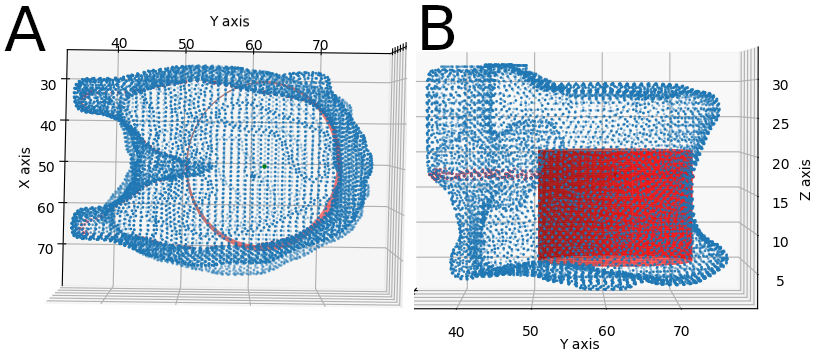
\includegraphics[width=5in]{Chapters/Chapter_HT_images/cyl_fit_channel_both.png}
  \caption{An illustration showing the problems that occur with vertebrae that have a distinctive vascular channel and the false cylinder fit that occurs.}
  \label{fig:cyl_channel}
\end{figure}

This was carried out using a set of scripts written in python and rely of having stl files describing the vertebral geometry.
The scripts work by finding the middle slice of a set of nodes that describe the vertebra.
From the middle slice the shape of the ellipse is formed.
Given that the alignment of the vertebrae is uniform, the mid point on the $y$ axis is found by searching for the node furthest away from the weighted center, $\pm$ 2 mm of the weighted centre.
This gives the $a$ measure of the ellipse description.
The $b$ measure is found by using a similar process - searching for the node furthest away from the centre on the $x$ axis, within $\pm$ 2 mm.
The $a$ and $b$ measures gave the shape of the ellipse and the height of the elliptic cylinder was found by raising and lowering the ellipse until a node in the middle $\pm$ 5 mm intersected the ellipse.
This defined the height of the ellipse.
The volume of the ellipse was found (V = $\pi a b h$, where $a$ and $b$ have been described and $h$ is the height) and compared to that of the total vertebral volume, shown in table~\ref{tab:vertebrae_vol_cyl}.
The percentage reduction in vertebral body volume, from total vertebral body volume to the fitted cylinder volume, varies significantly and is due to changes to the vertebral shape outside of the main vertebral body portion.
For example, G19-11 L1 was a degenerate vertebrae with extra bone growth at the anterior limits of the vertebral body.
Other large changes were due to the size of the pedicles, where larger vertebrae (G41-11) had proportionally larger pedicles.

\begin{table}[ht!]
\centering
  \caption{Vertebral body volume compared to the volume of the fitted cylinder.}
	\label{tab:vertebrae_vol_cyl}
  \begin{tabular}{c |c|c|c}
	  Specimen & Total Vertebral  & Fitted Cylinder & Change in Volume\\ 
	  &Body Volume (mm$^3$)&Volume (mm$^3$) &(\%)\\ \hline \hline
	  G17-11\_L1  & 31229 & 17490 & -44\\
	  G17-11\_L2  & 31789 & 20551 & -35\\
	  G17-11\_L3  & 33519 & 22014 & -34\\
	  G17-11\_L4  & 35123 & 22796 & -35\\
	  G17-11\_L5  & 31189 & 22254 & -28\\
	  G19-11\_L1  & 33835 & 17420 & -48\\
	  G21-11\_L1  & 45866 & 31073 & -32\\
	  G21-11\_L2  & 53695 & 34470 & -36\\
	  G21-11\_L3  & 56003 & 36750 & -34\\
	  G41-11\_L1  & 35137 & 22231 & -37\\
	  G41-11\_L2  & 36791 & 23837 & -35\\
	  G41-11\_L3  & 39909 & 26036 & -35\\
	  G41-11\_L4  & 43357 & 25612 & -41\\
	  G41-11\_L5  & 45606 & 26936 & -41\\
	  \hline
  \end{tabular}

\end{table}

The effect of this change on the relationship between cement fill and change in augmentation stiffness was identified and is shown in figure~\ref{fig:cyl_fit_comparison}.
While there was a change in the relationship, a clear trend between the cement fill percentage and change in stiffness for the majority of the vertebrae is still not evident without including other factors (described in Section~\ref{sec:aug_stiffness_res}).

\begin{figure}[ht!]
  \centering
  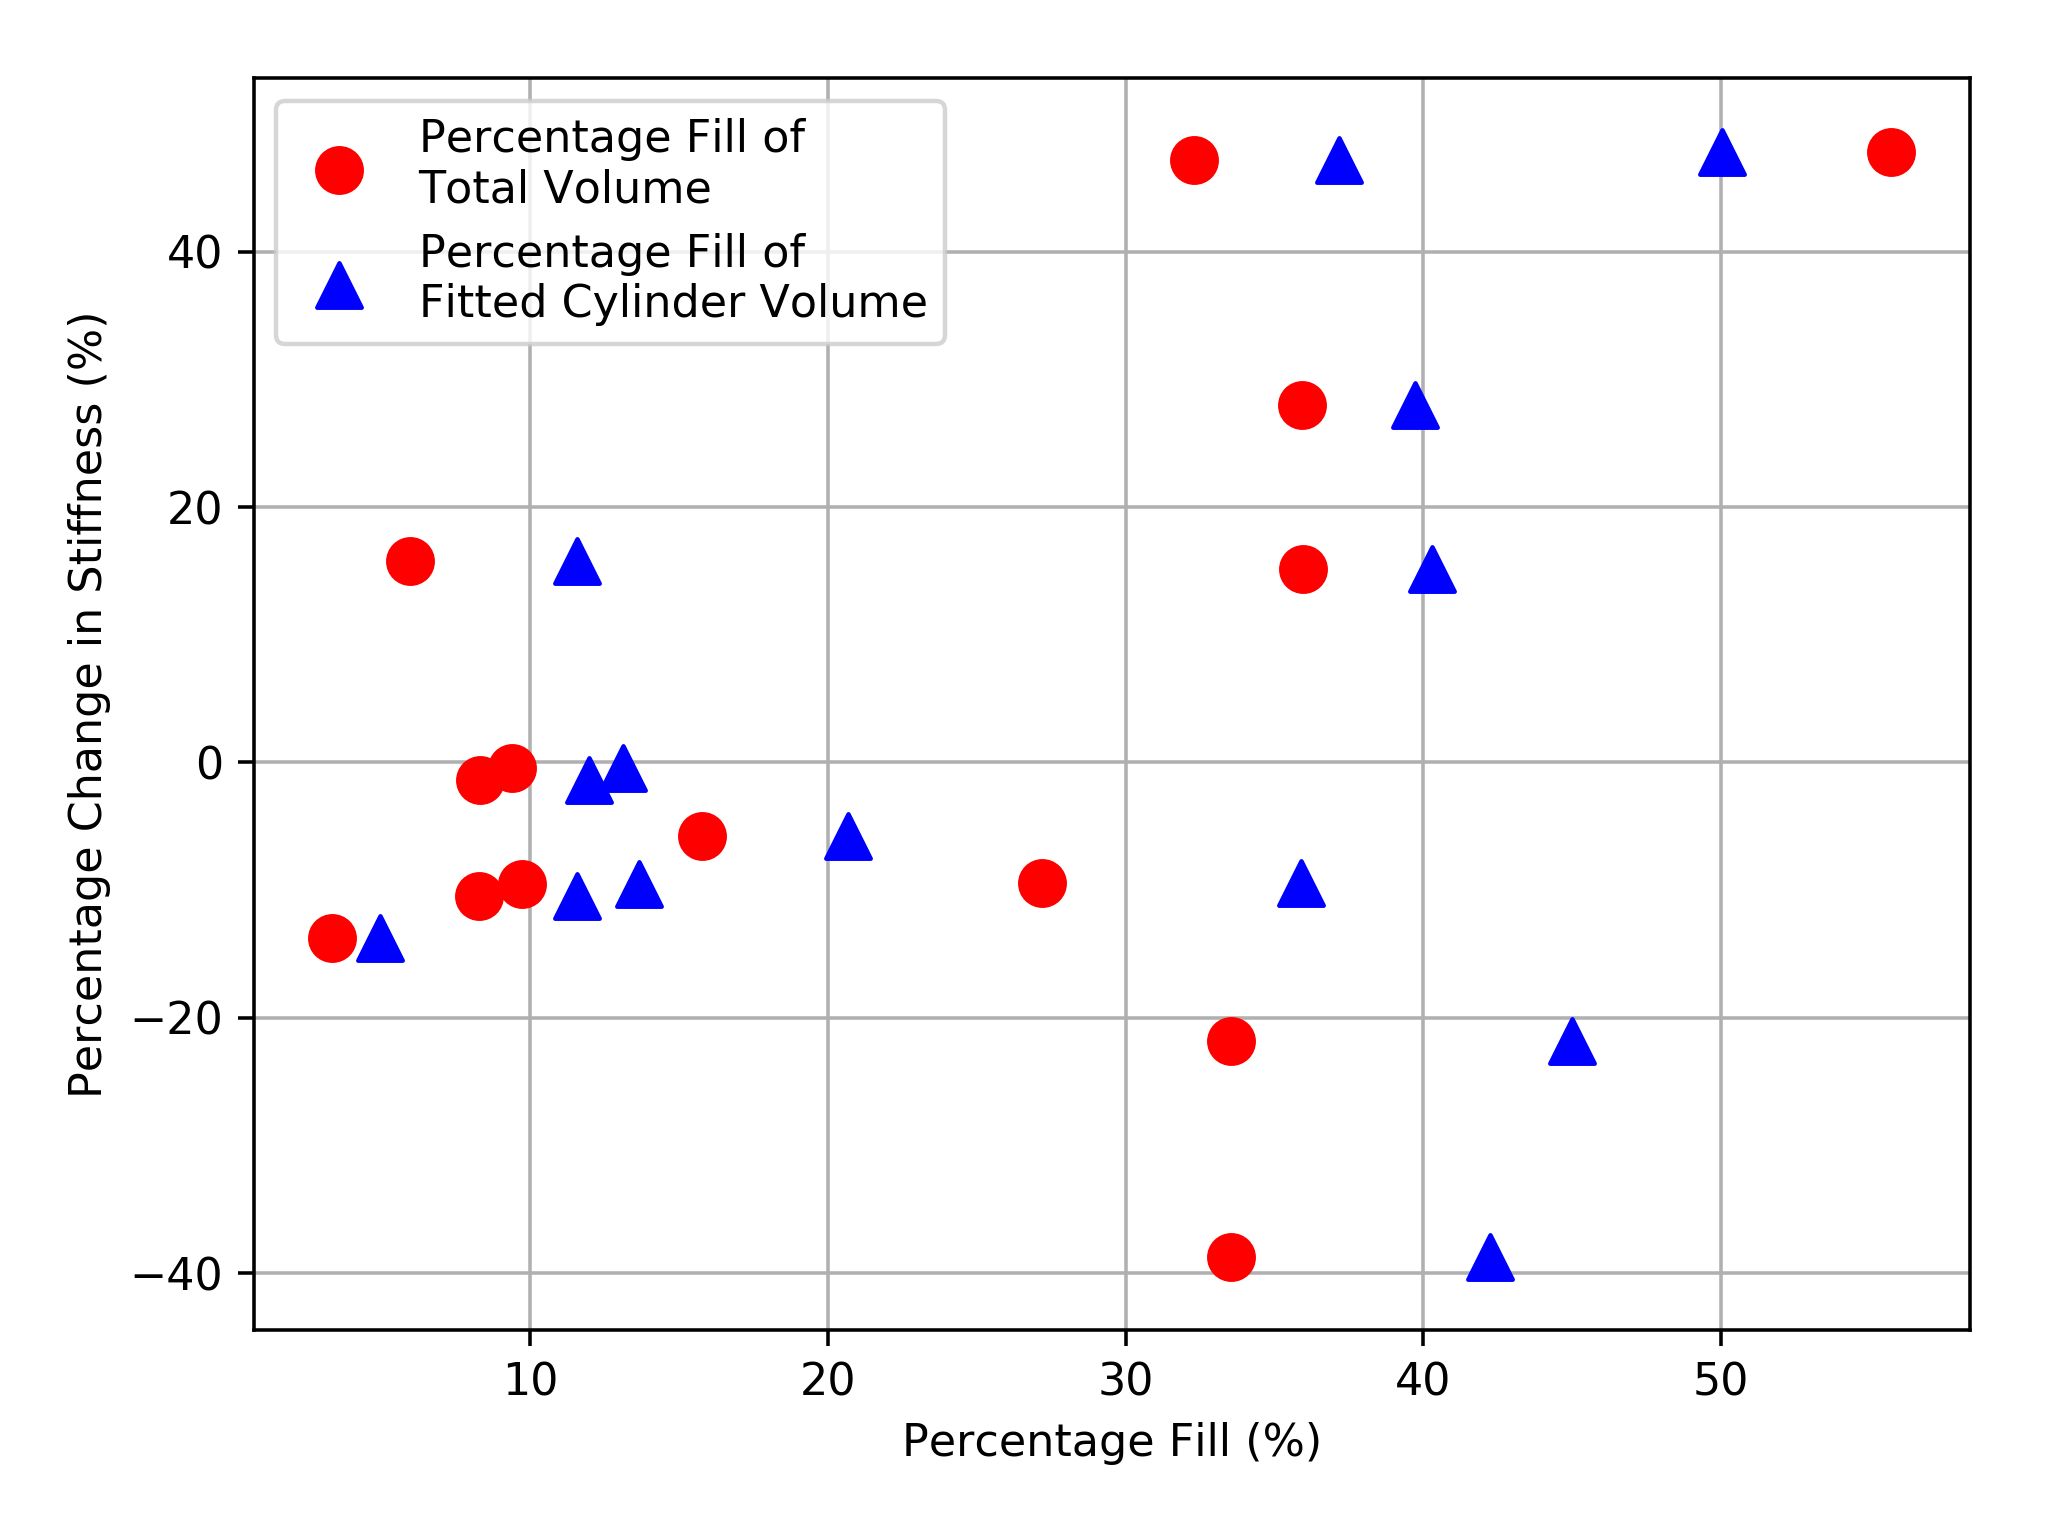
\includegraphics[width=.7\textwidth]{Chapters/Chapter_HT_images/cyl_fit_comparison.png}
  \caption{The effect of using the fitted cylinder as a measure of vertebral body volume, on the relationship between augmentation fill volume and change in stiffness following augmentation. The red points show the relationship using the total vertebral volume, with the relationship using the fitted cylinder shown in blue.}
  \label{fig:cyl_fit_comparison}
\end{figure}

\section{Results}


\subsection{Experimental Loading Results}

\subsubsection{Non-augmented Stiffness Results}

\subsubsection{Augmented Stiffness Results}\label{sec:aug_stiffness_res}

A strong relationship was found between the percentage fill achieved and the bone volume fraction of the vertebra, where a reduced density of bone resulted in larger quantities of cement being injected into the vertebra before cement leakage occurred.
This relationship can be seen in figure~\ref{fig:cmt_fill_vs_bvtv}.

\begin{figure}[ht!]
  \centering
  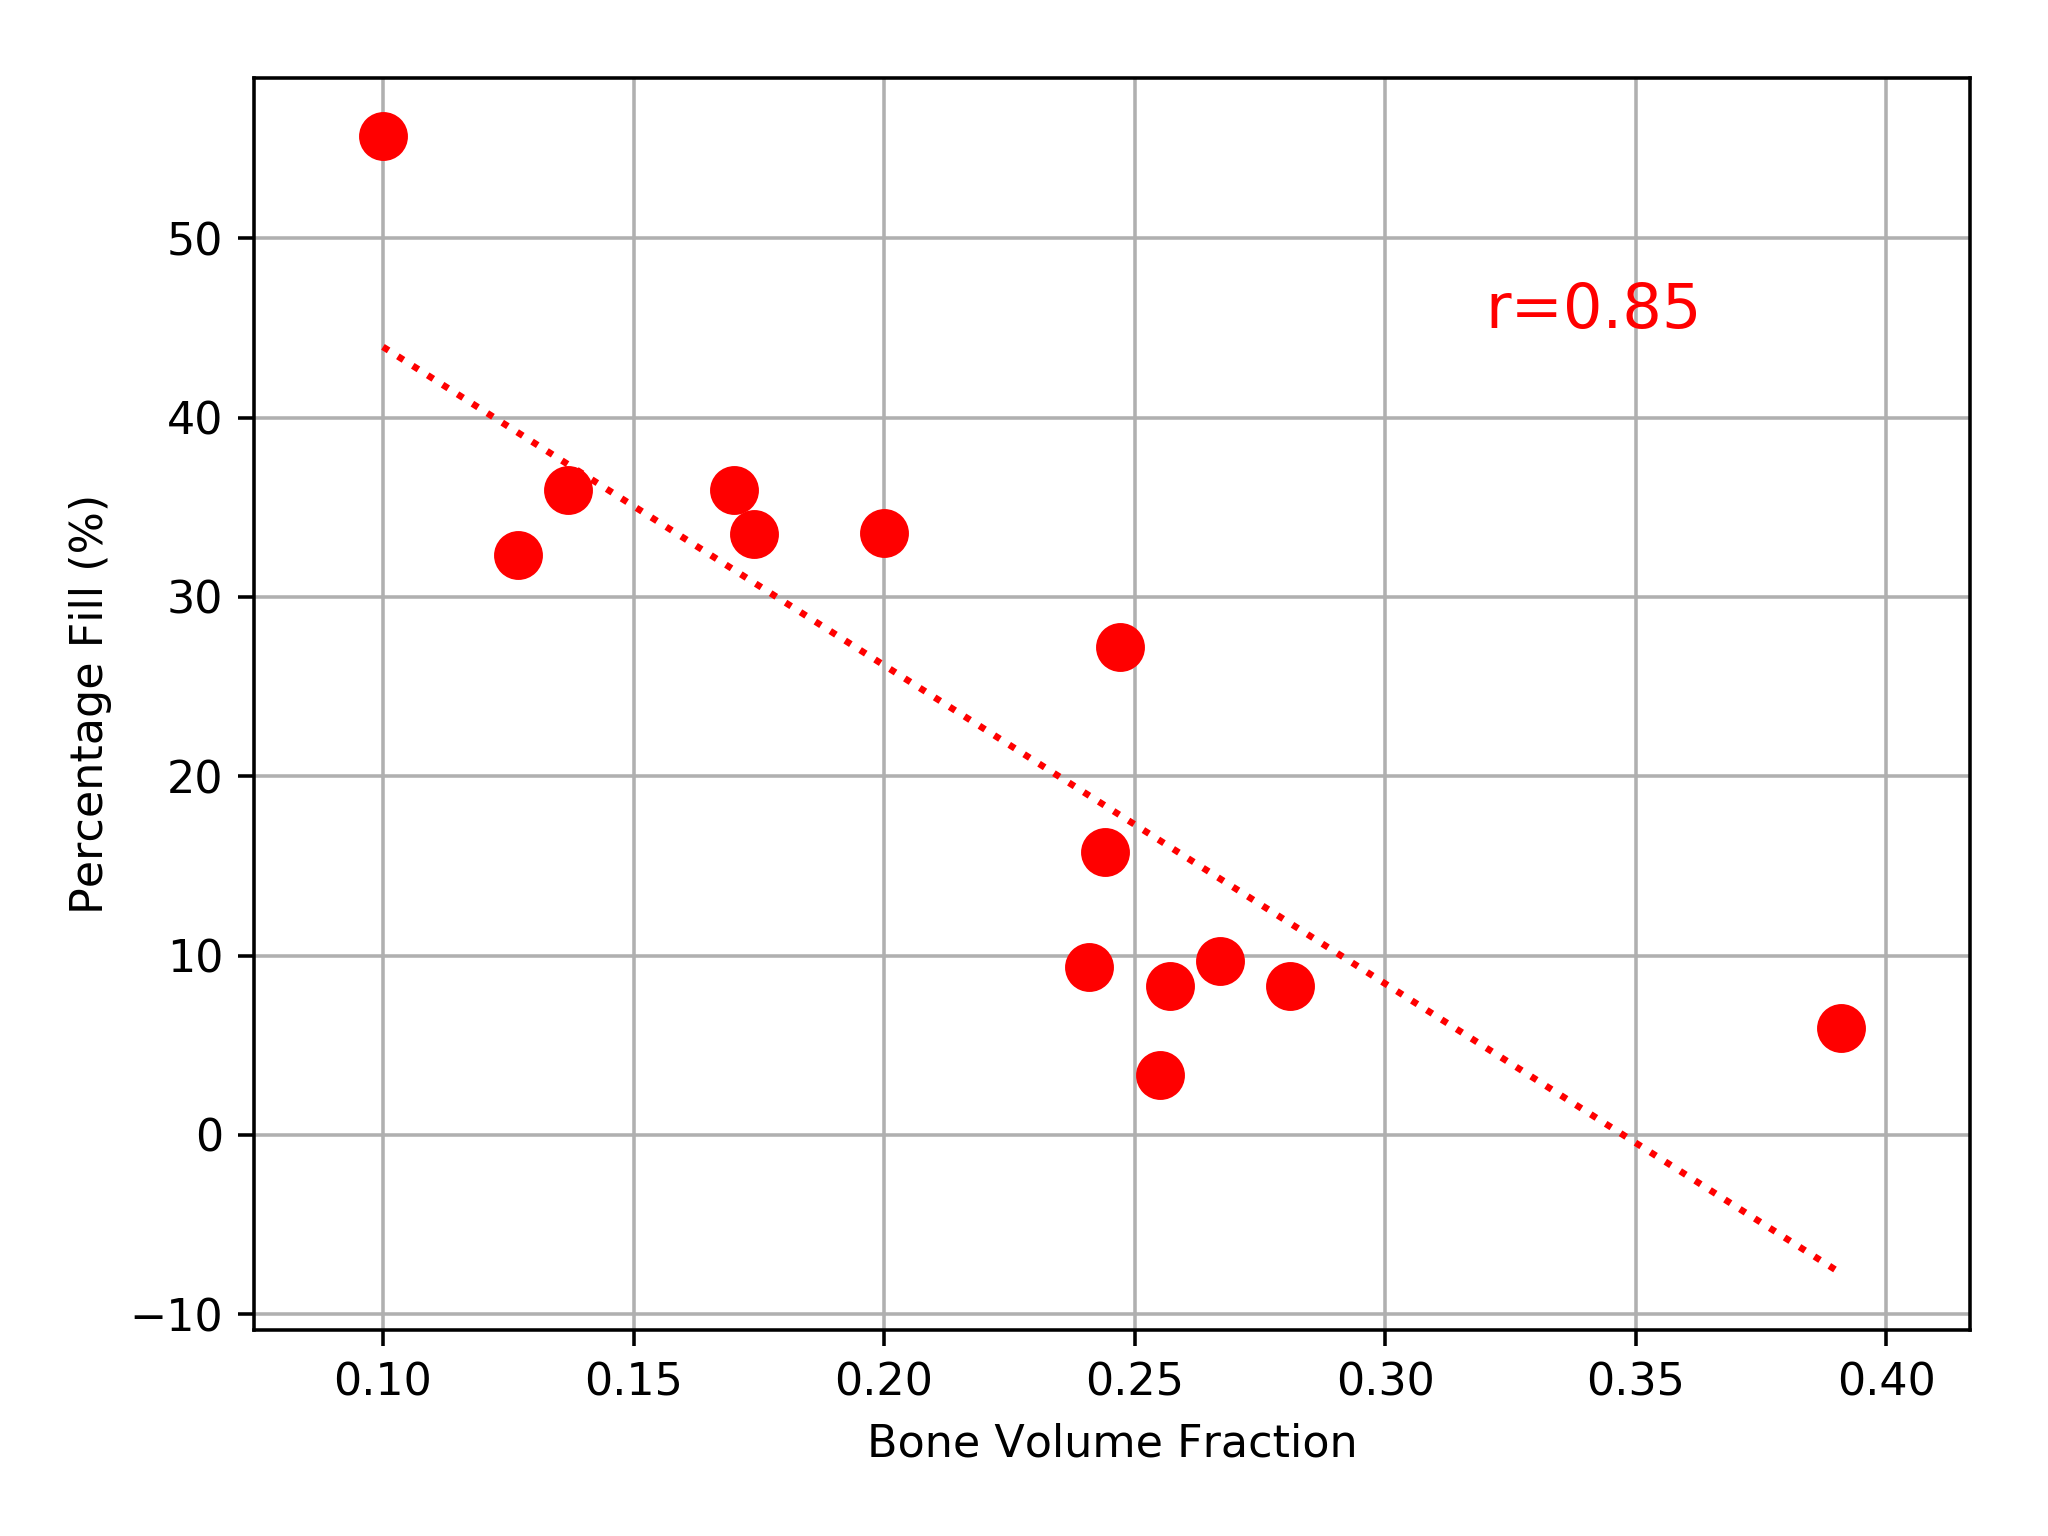
\includegraphics[width=.7\textwidth]{Chapters/Chapter_HT_images/cmt_fill_vs_bvtv.png}
	\caption{The relationship between the percentage cement fill of the total vertebral volume  achieved through the augmentation procedure and the bone volume fraction value for each vertebra. }
  \label{fig:cmt_fill_vs_bvtv}
\end{figure}

There was not a clear relationship found between the cement fill of the total vertebral volume and the resulting change in stiffness following augmentation for the set of vertebrae on the whole.
However, trends could be seen when splitting vertebrae into groups with: \textit{a)} dispersed volumes of injected cement and \textit{b)} concentrated volumes of cement.
This can be seen in figure~\ref{fig:cmt_fill_vs_ch_stiff} where a trend ($r=0.83$) can be seen between the percentage fill of the total vertebral volume and the percentage change in stiffness for those vertebrae with concentrated volumes of cement.

\begin{figure}[ht!]
  \centering
  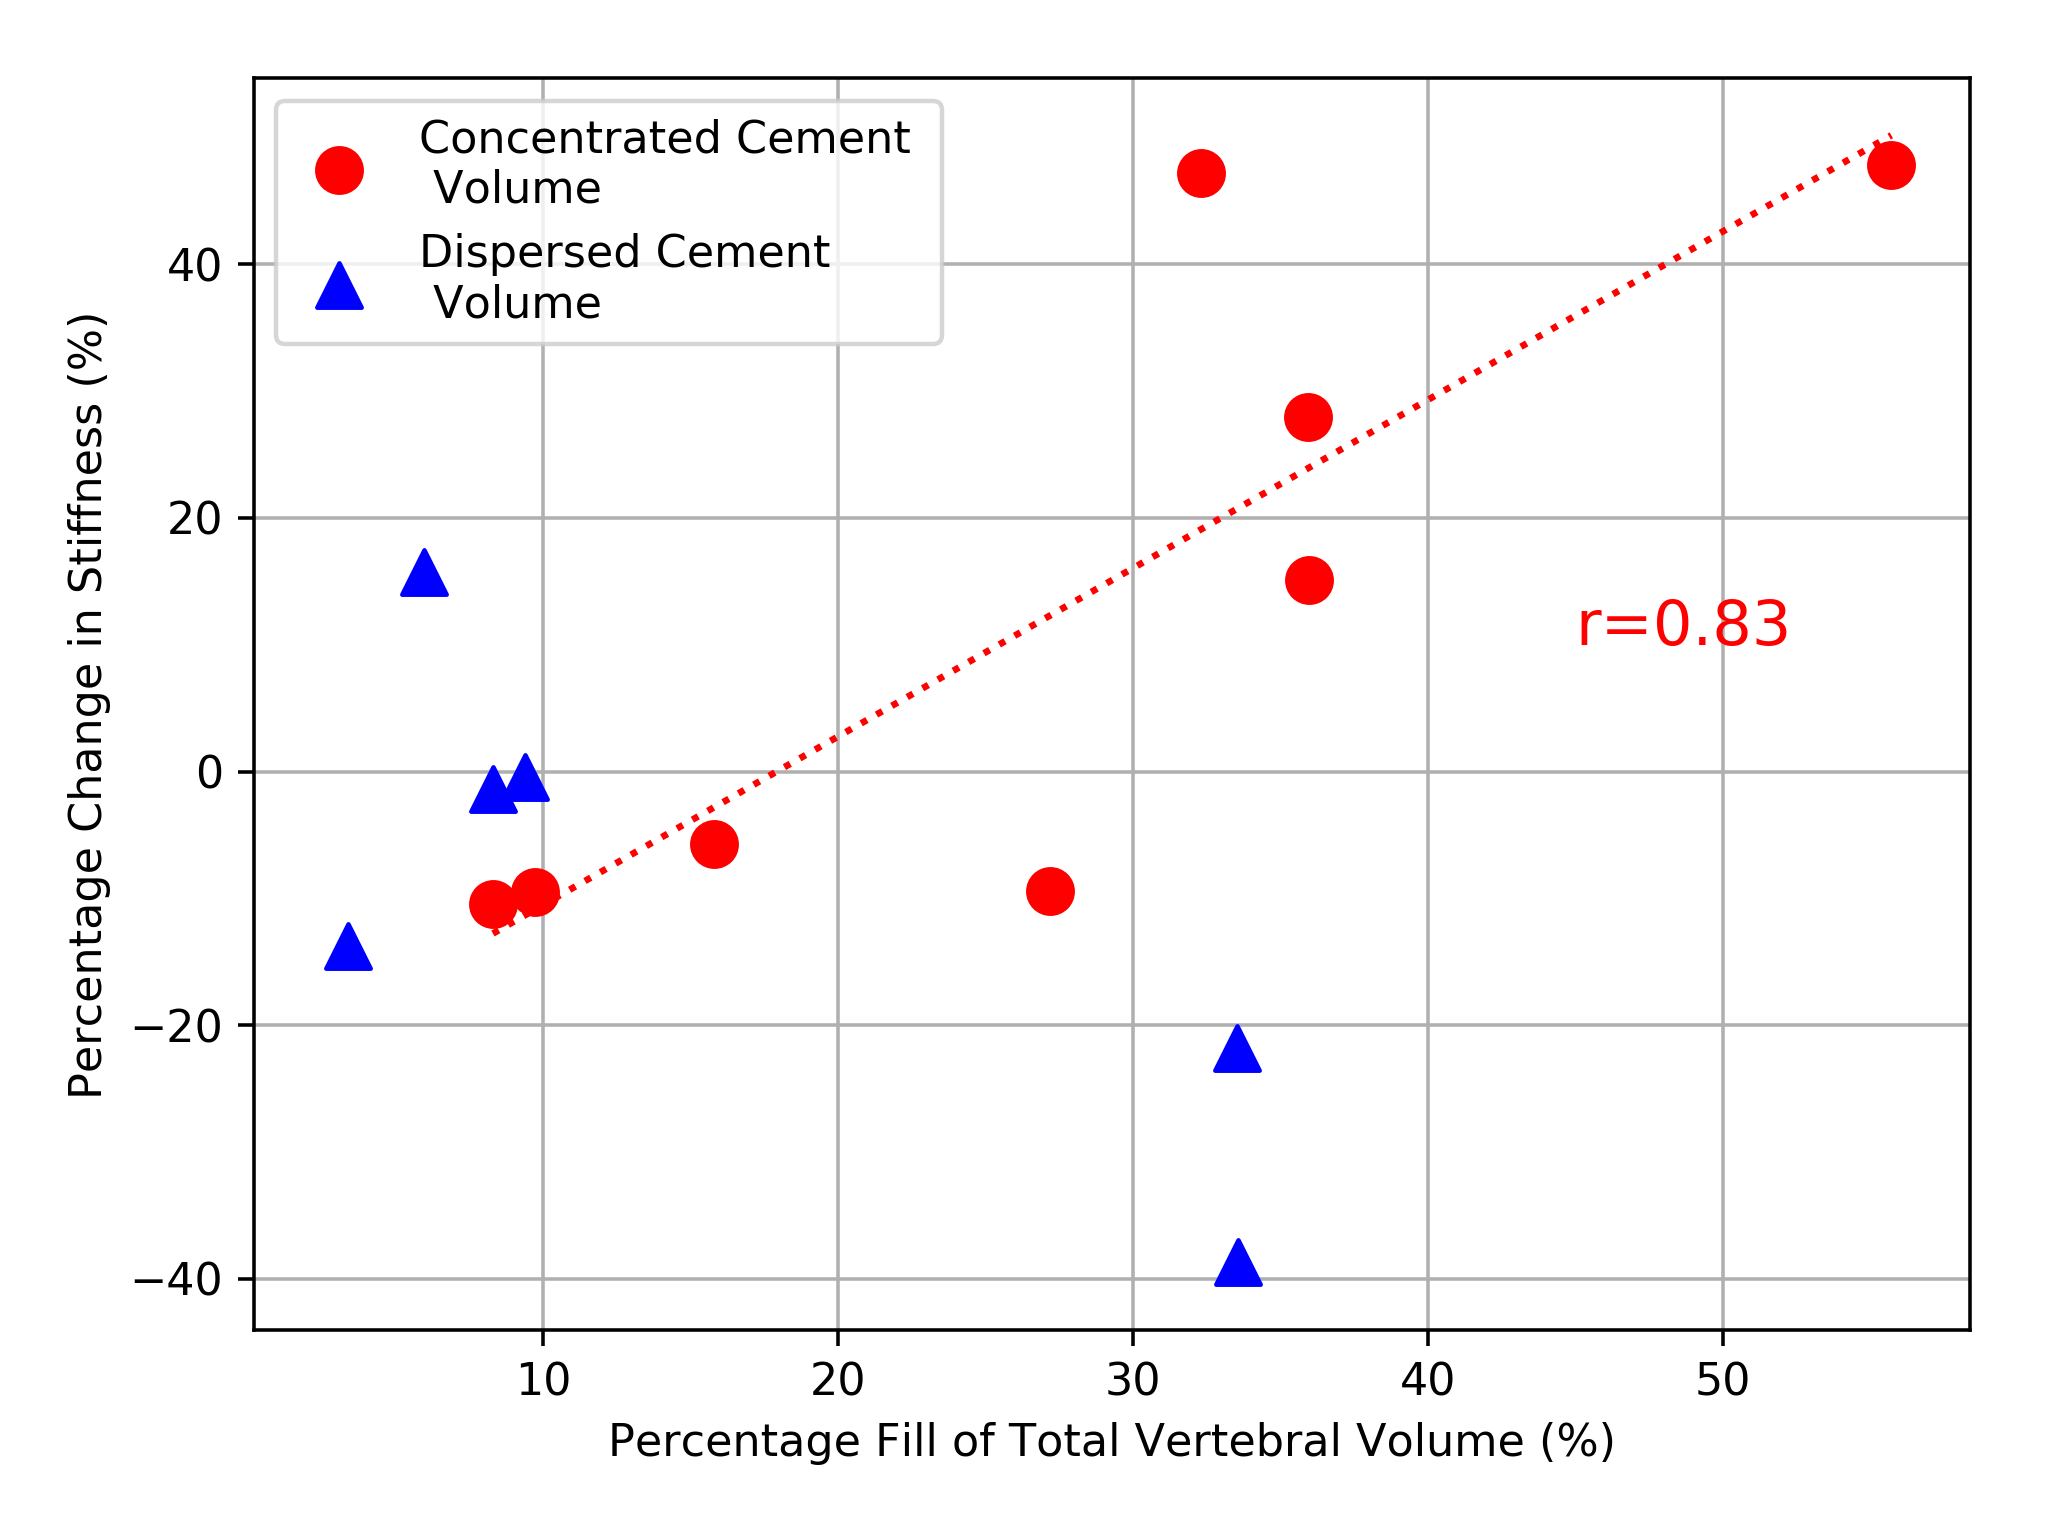
\includegraphics[width=.7\textwidth]{Chapters/Chapter_HT_images/Aug_cmt_fill_vs_ch_stiff.png}
	\caption{The relationship between the percentage fill of the total vertebral volume and the percentage change in the vertebral stiffness following augmentation. The line and \textit{r} value are for the red points where the cement volume was characterised as concentrated. The remaining blue points indicated the vertebra where the cement volume was characterised as dispersed.}
  \label{fig:aug_cmt_fill_vs_ch_stiff}
\end{figure}

\subsection{Experimental Augmentation}


\begin{figure}[ht!]
  \centering
  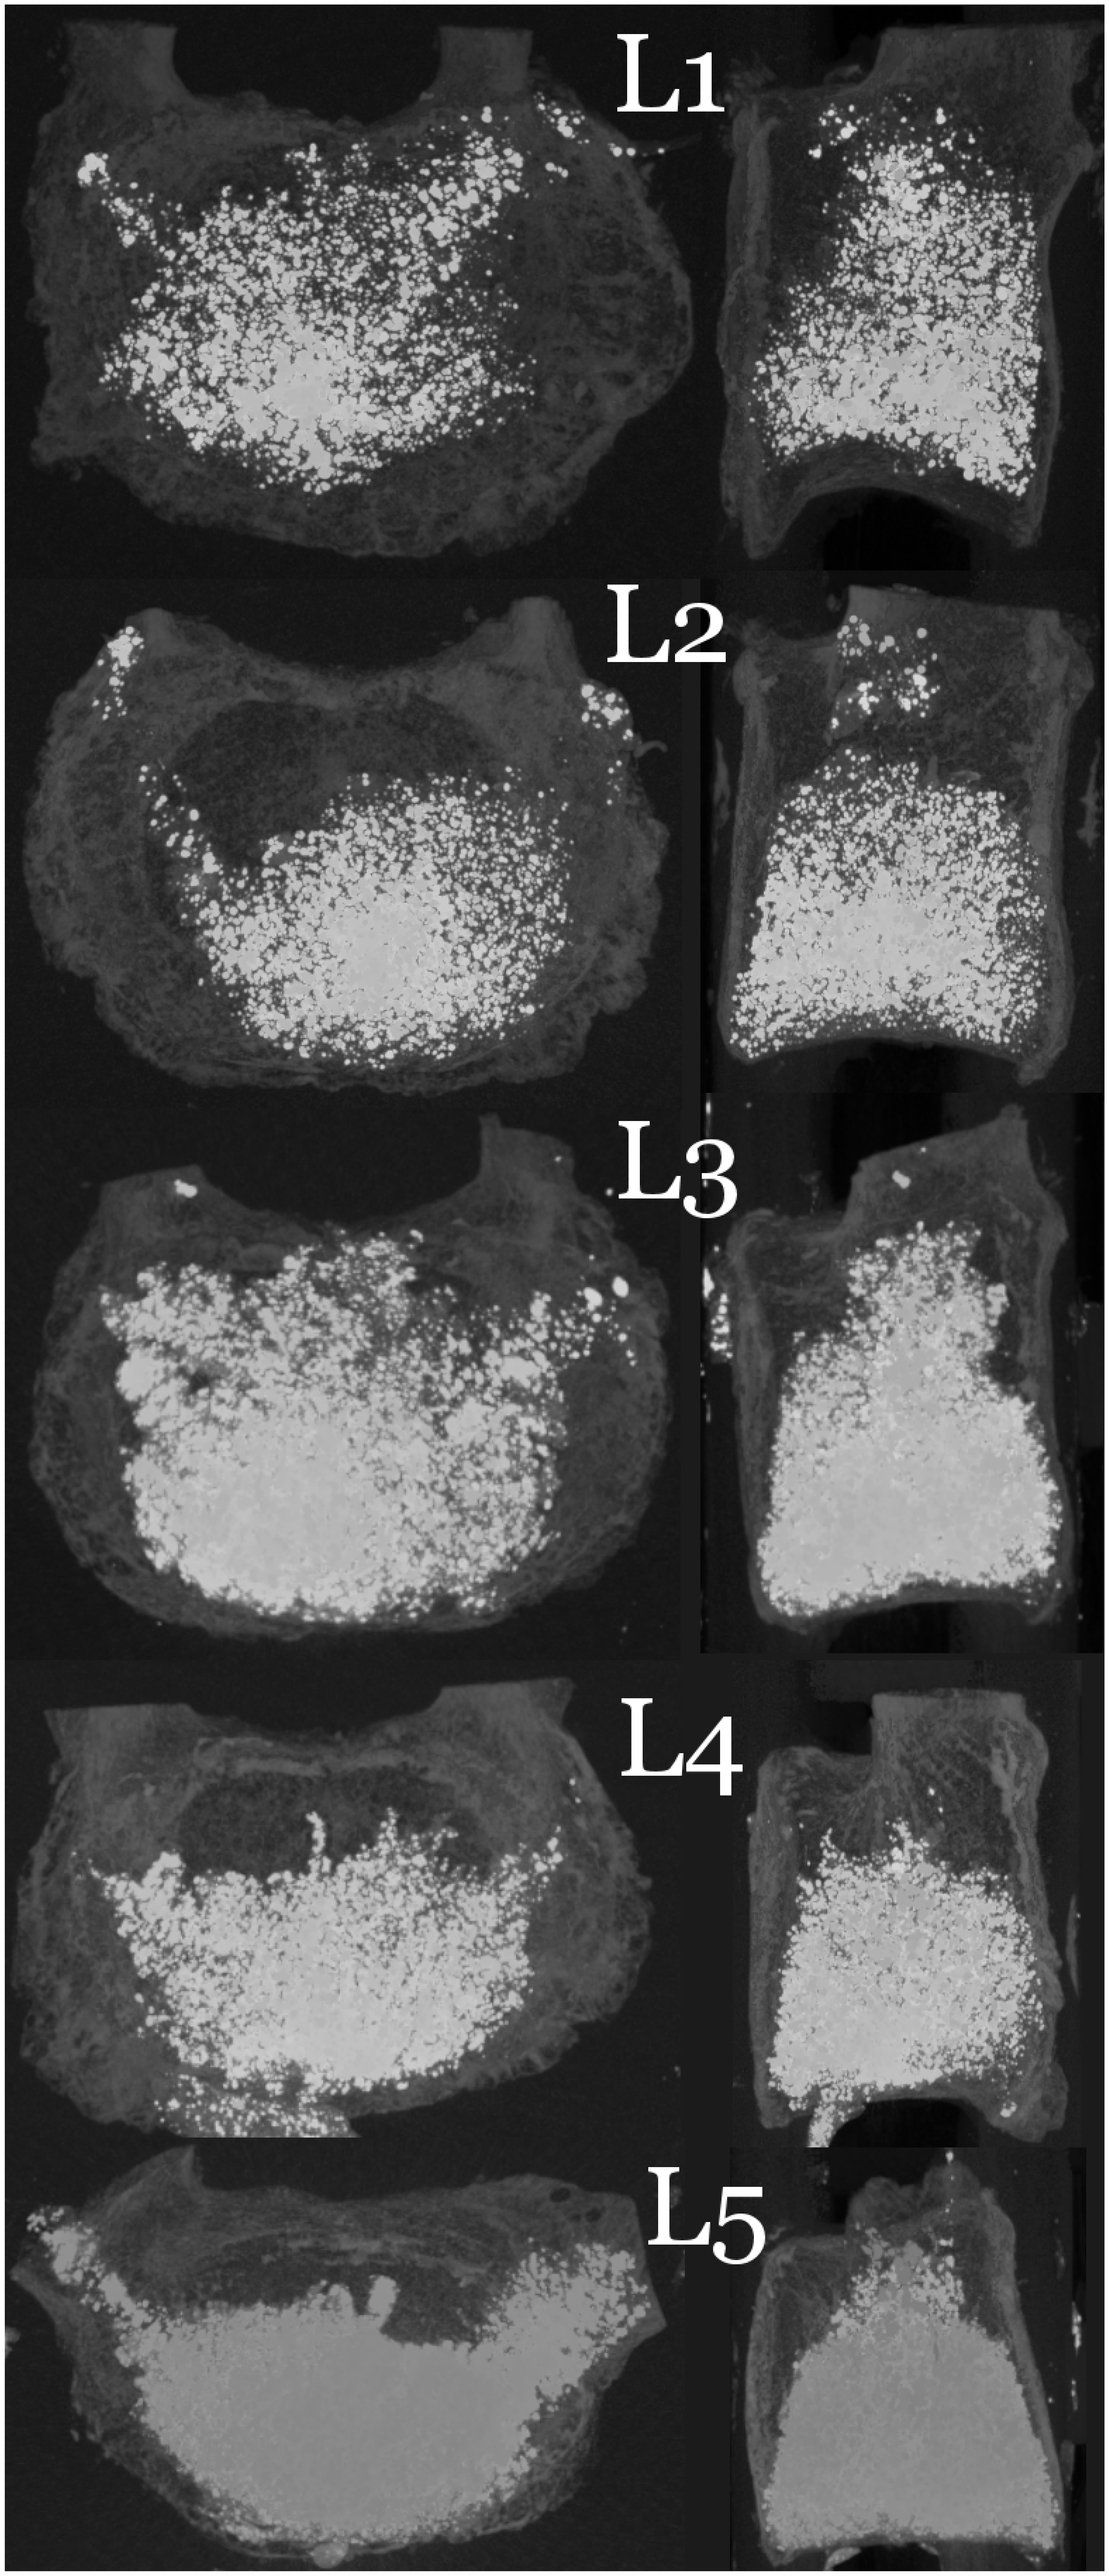
\includegraphics[width=\textwidth]{Chapters/Chapter_HT_images/G17-11_projections.eps}
	\caption{Transverse and sagittal 3D projection views of the G17-11 spine following augmentation, with the cement region being the brighter material in the vertebral body. The L1 vertebra is defined as having a dispersed volume of cement while the remaining L2, L3, L4, L5 vertebrae have concentrated volumes of cement.}
  \label{fig:G17-11_projection}
\end{figure}

\begin{figure}[ht!]
  \centering
  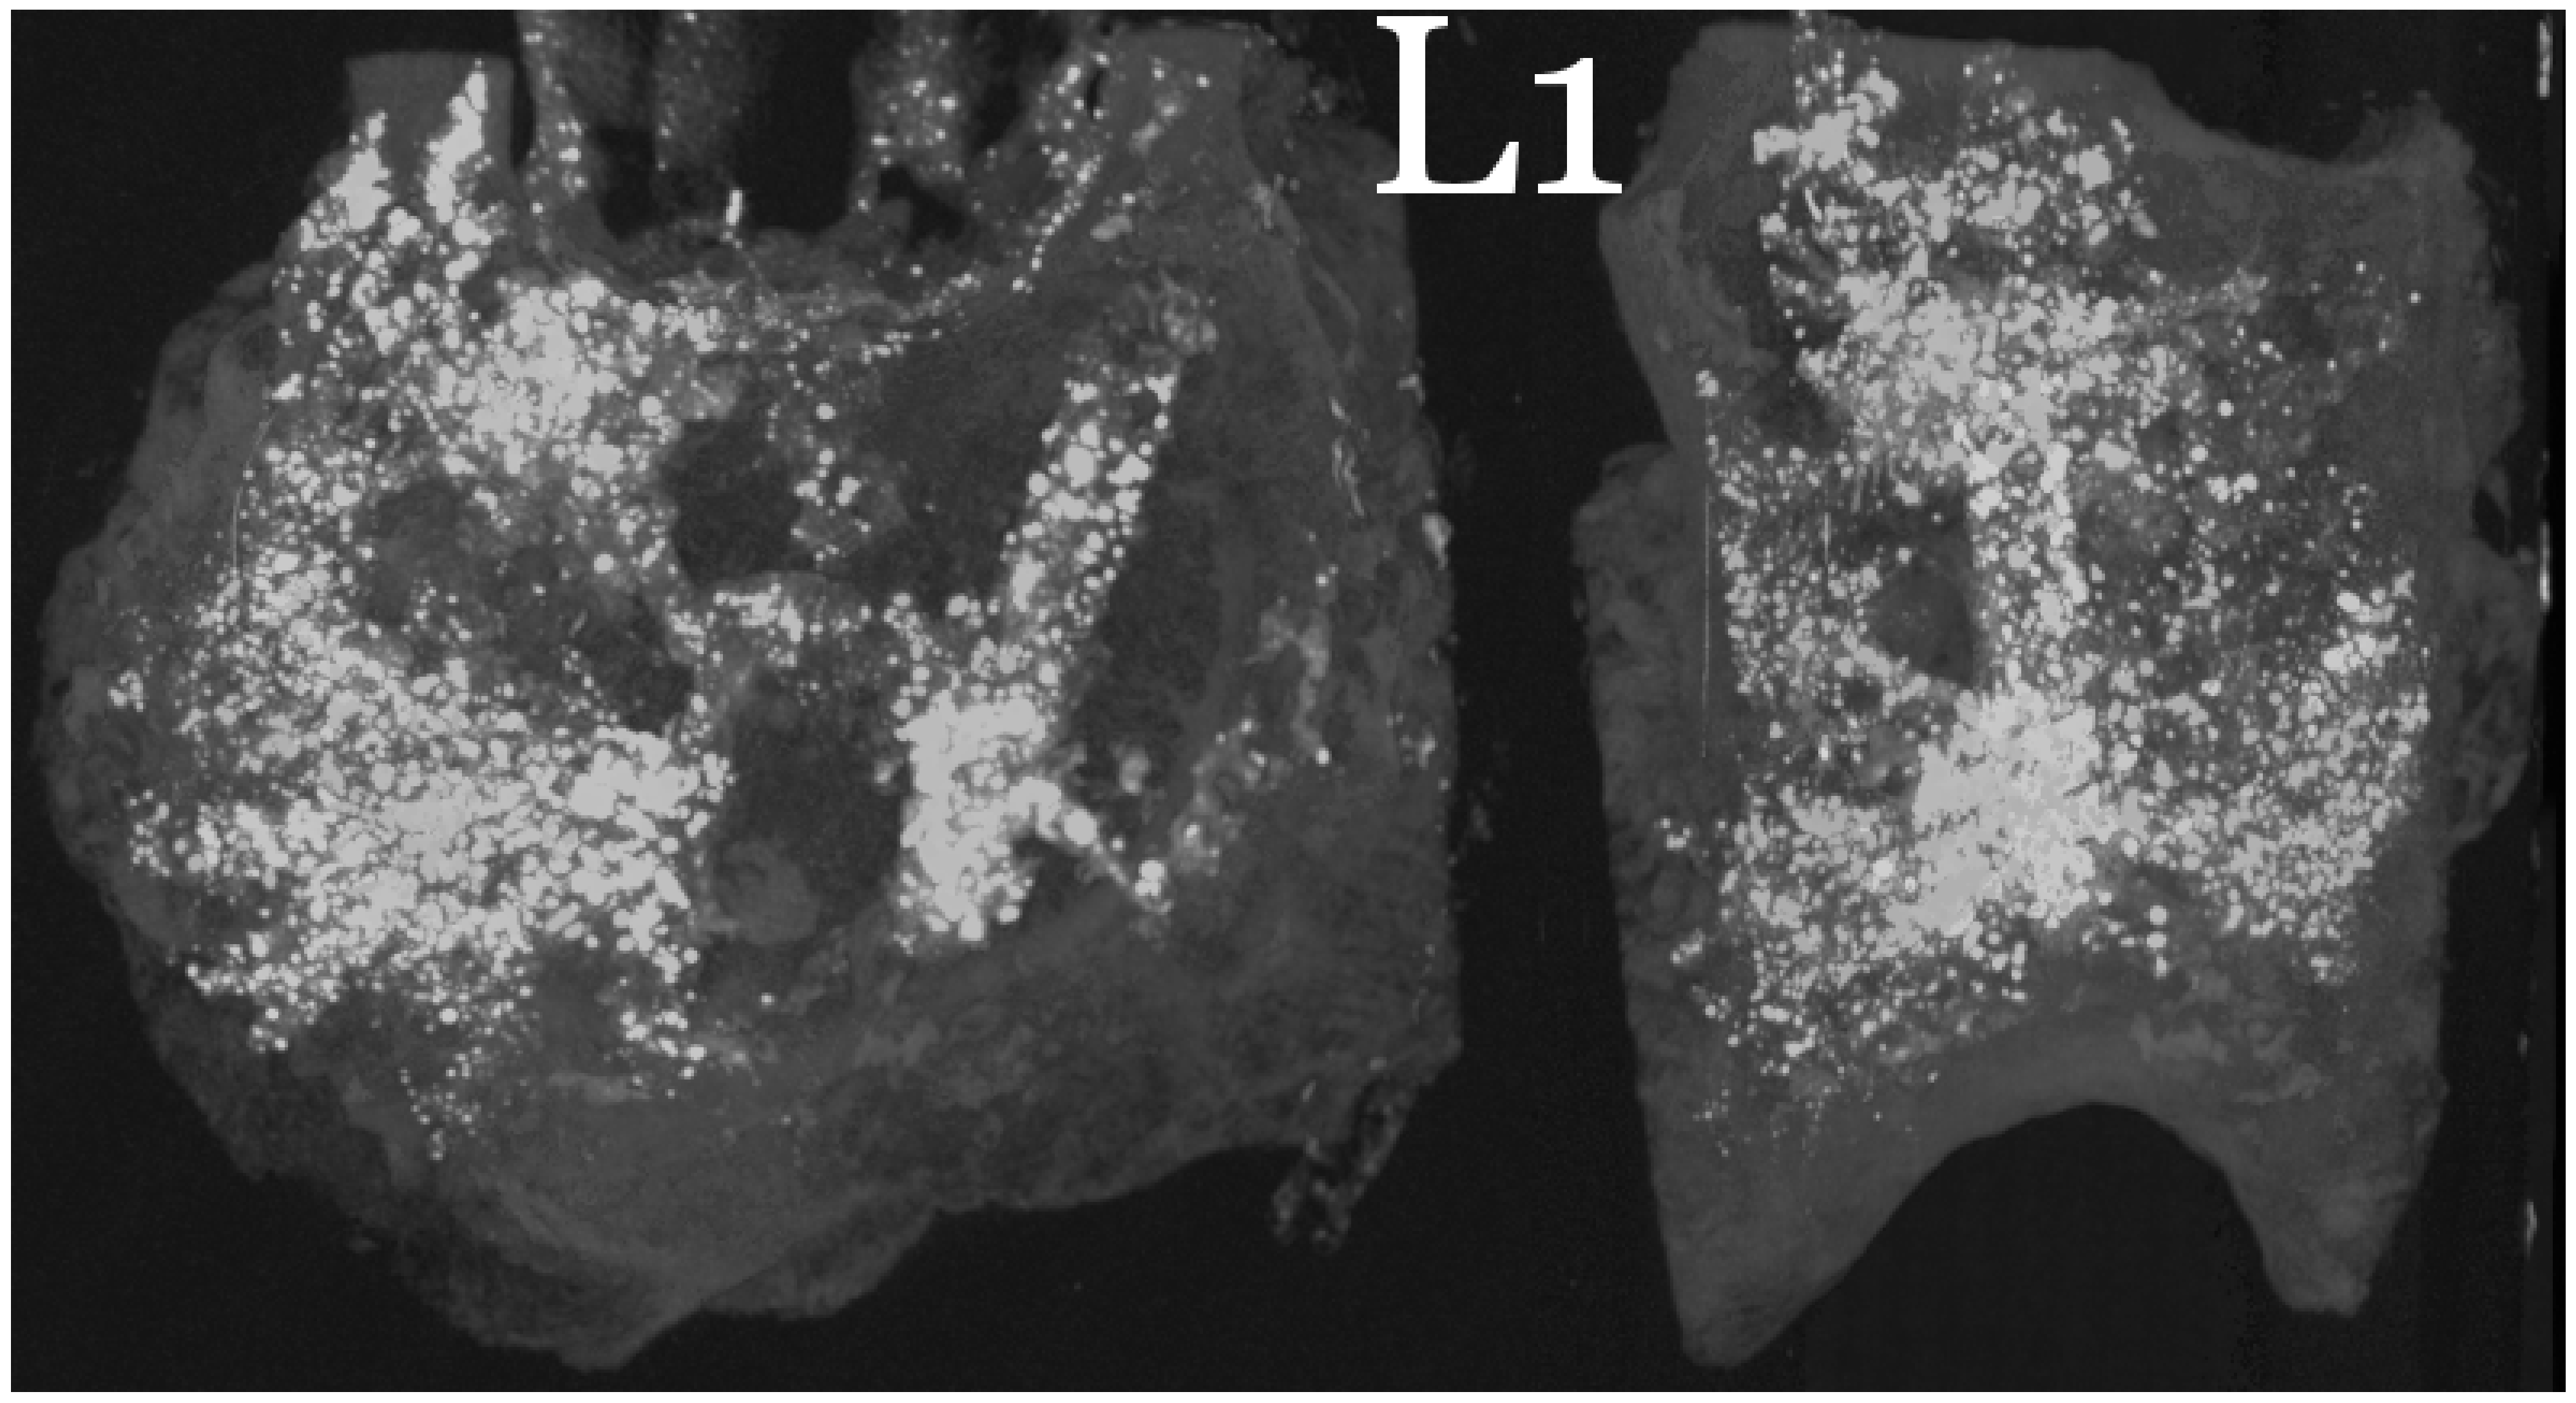
\includegraphics[width=\textwidth]{Chapters/Chapter_HT_images/G19-11_projections.eps}
	\caption{Transverse and sagittal 3D projection views of the G19-11 spine following augmentation, with the cement region being the brighter material in the vertebral body. The vertebra is defined as having a dispersed volume of cement.}
  \label{fig:G19-11_projection}
\end{figure}

\begin{figure}[ht!]
  \centering
  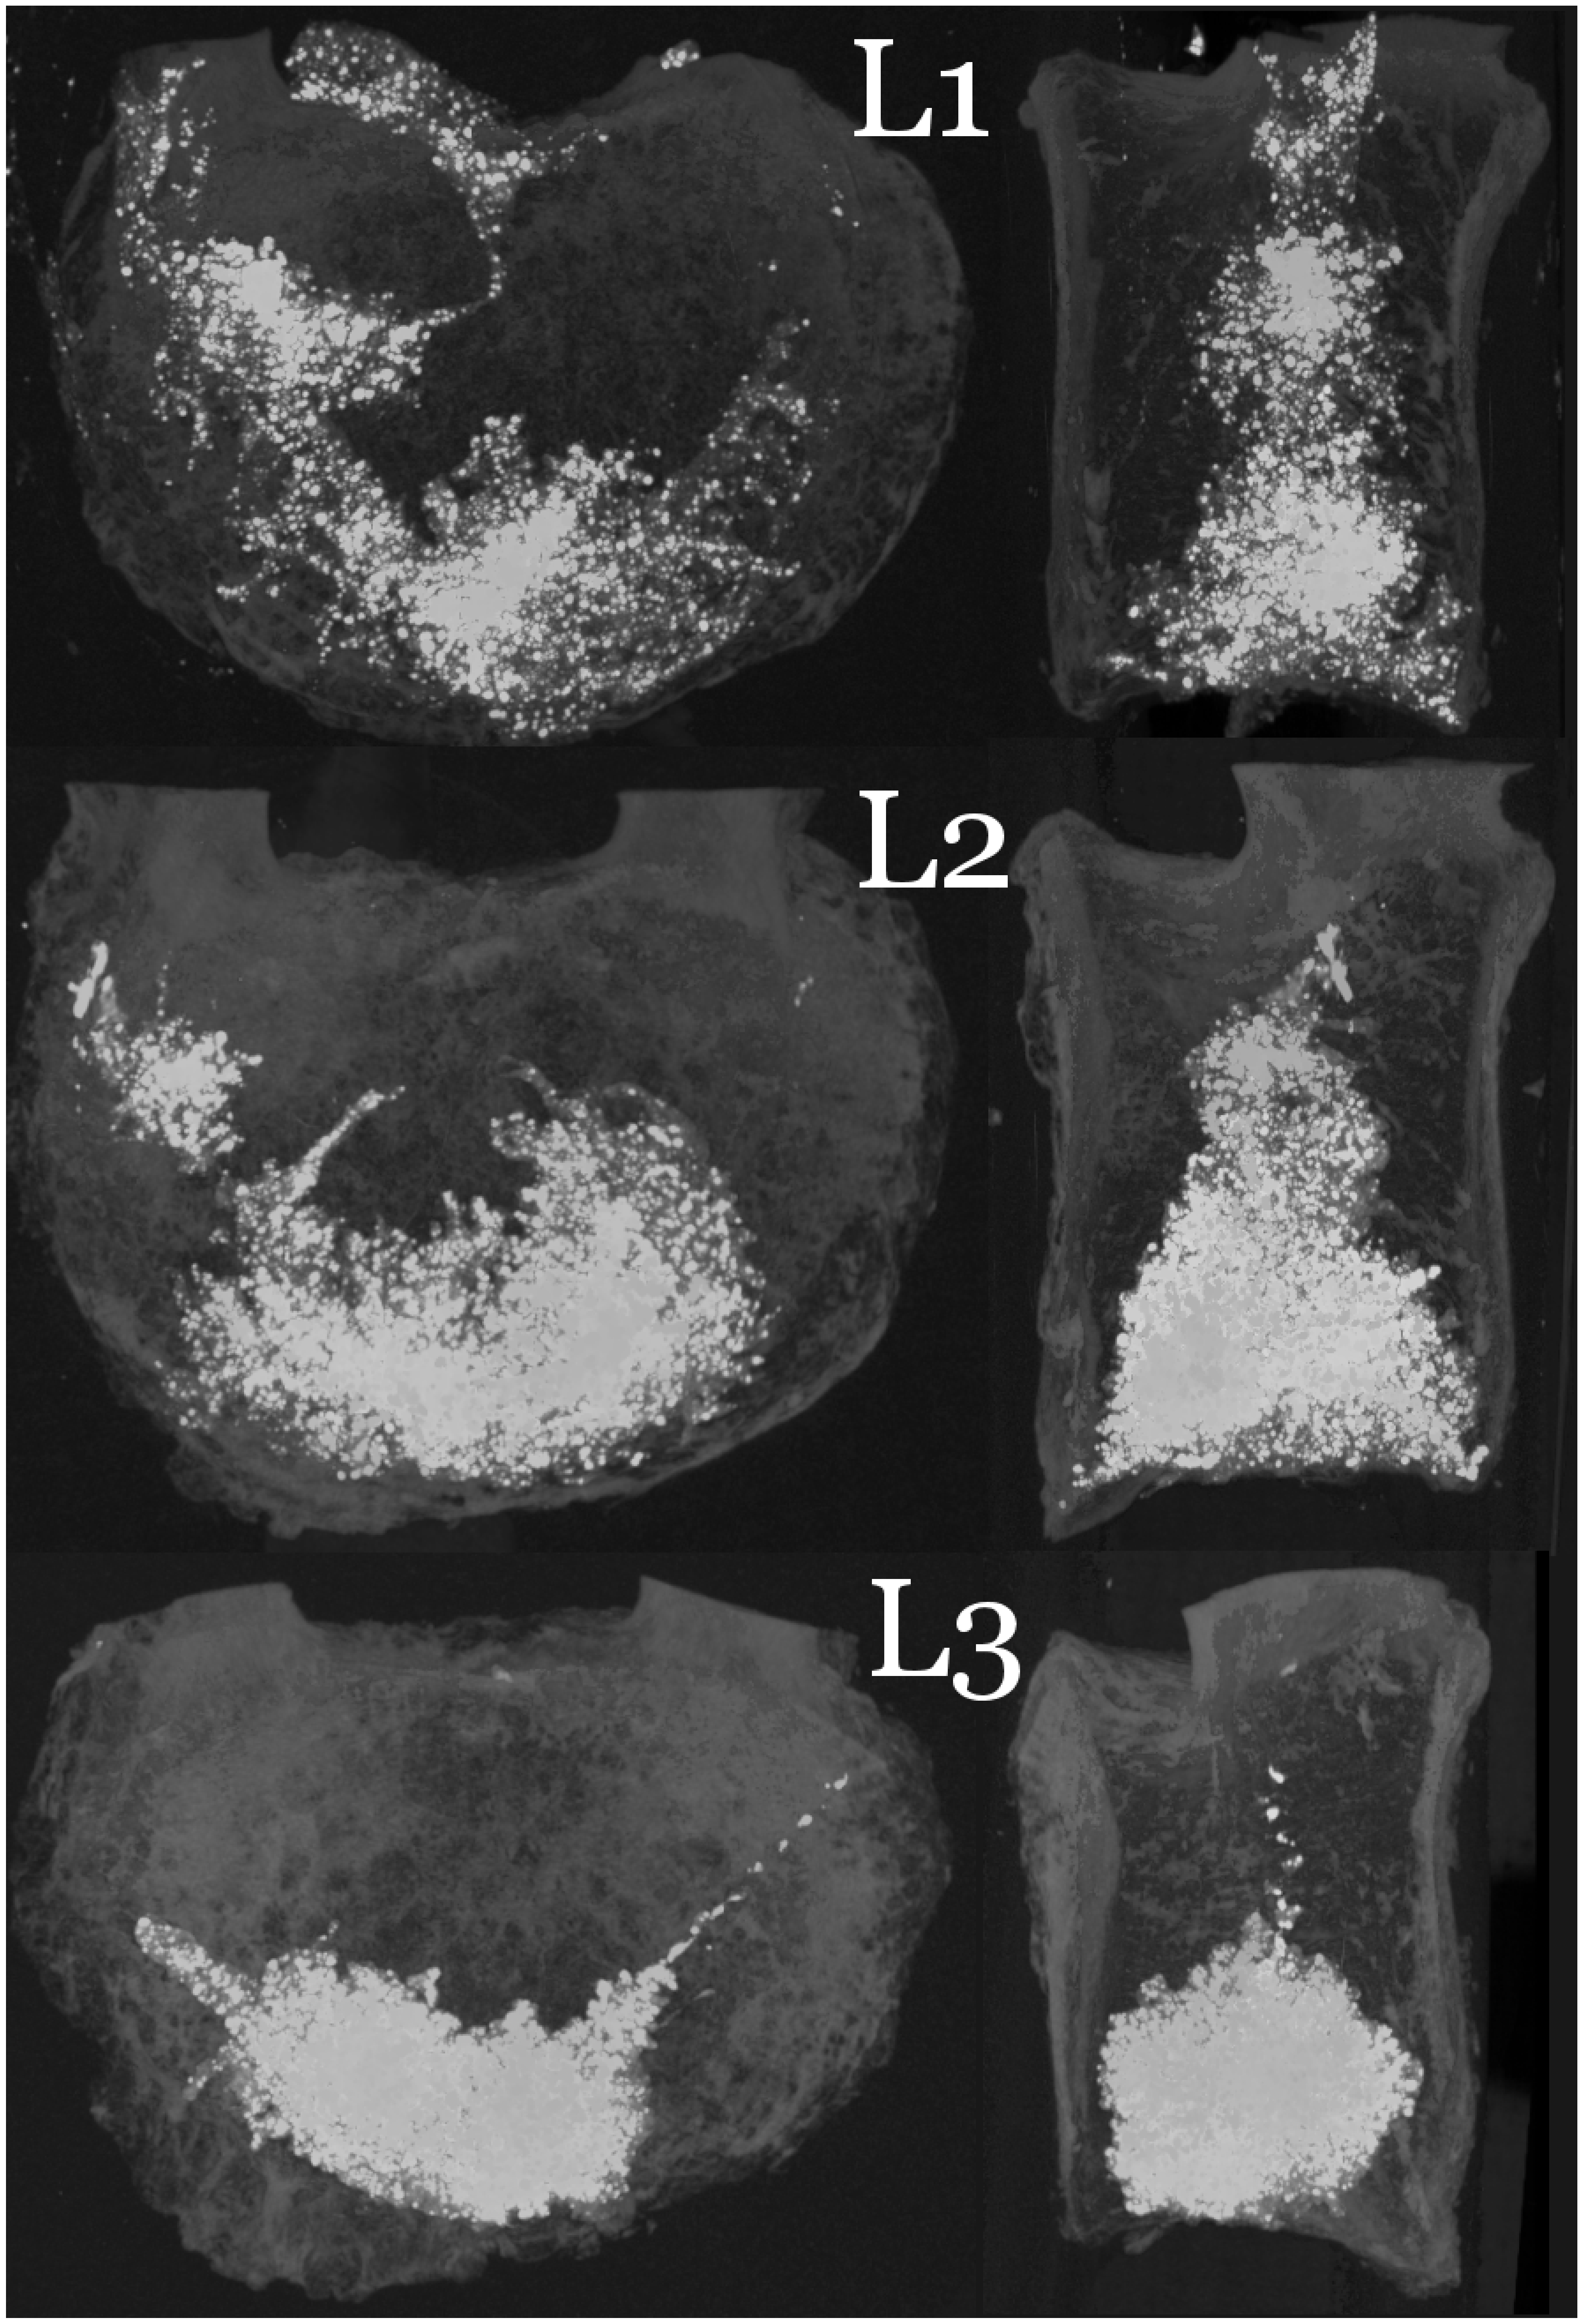
\includegraphics[width=\textwidth]{Chapters/Chapter_HT_images/G21-11_projections.eps}
	\caption{Transverse and sagittal 3D projection views of the G21-11 spine following augmentation, with the cement region being the brighter material in the vertebral body. The L1 vertebra is defined as having a dispersed volume of cement while the remaining L2 and L3 vertebrae have concentrated volumes of cement.}
  \label{fig:G21-11_projection}
\end{figure}

\begin{figure}[ht!]
  \centering
  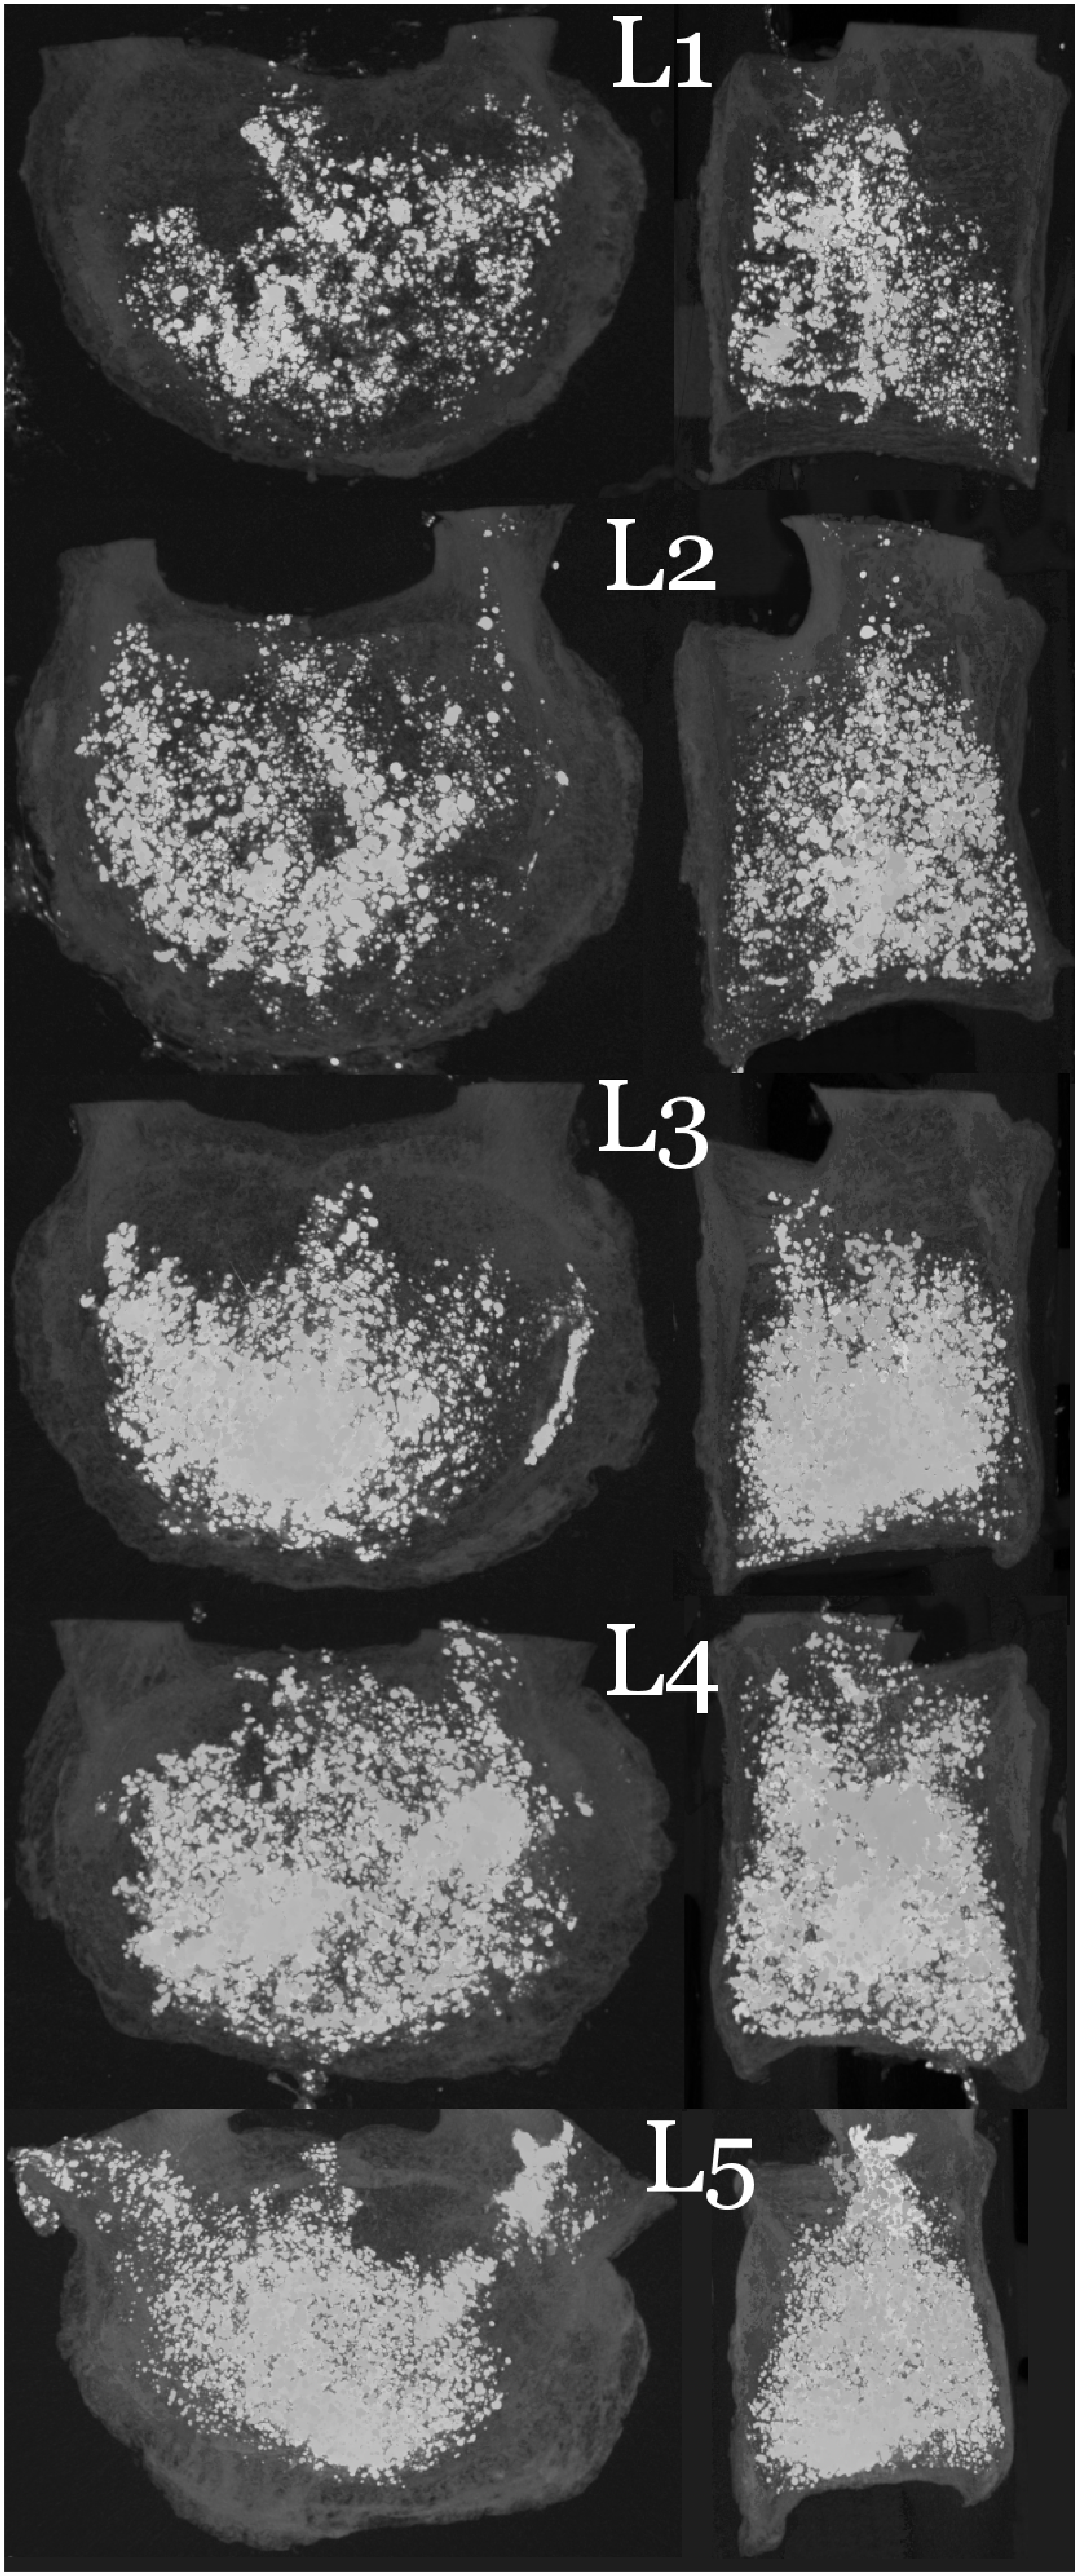
\includegraphics[width=\textwidth]{Chapters/Chapter_HT_images/G41-11_projections.eps}
	\caption{Transverse and sagittal 3D projection views of the G41-11 spine following augmentation, with the cement region being the brighter material in the vertebral body. The L1, L2 and L5 vertebrae are defined as having a dispersed volume of cement while the remaining L3 and L4 vertebrae have concentrated volumes of cement.}
  \label{fig:G17-11_projection}
\end{figure}

\subsection{Computational Results}

\subsubsection{Non-augmented Model Results}

\subsubsection{Augmented Model Results}

\section{Discussion}





\subsection{Experimental Results}

Experimentally there was large variation seen in the results, in terms of material properties (BV/TV values), geometry and response to loading.

\subsection{Limitations Regarding Specimen Numbers \& Vertebral Features}

One of the main limitations to the study is the numbers of vertebrae included in in the set.
Having four human spines with a limited number of lumbar vertebrae available from each spine, meant that only 14 out of a possible 20 vertebrae were able to be tested.
This meant that there was a skew towards the top of the lumbar section with limited numbers of L4 and L5 vertebrae.
Such skews to the data set have effects to any statistics applied to the data set and will be discussed more thoroughly in the PCA discussion chapter in Section~\ref{pca_disc}.
More relevant to modelling the vertebrae is the effect this has on the determination and optimisation of the greyscale conversion factor.
The large change in geometry from L4 to L5, rather that the gradual change between L1 to L4, introduces questions about the response to loading (and augmentation) for this vertebra in particular and how it differs from other levels.
A resolution to this limitation would be to increase the specimen numbers and look at vertebral levels in isolation; identifying level specific differences and properties.
Variation at different vertebral levels may require level specific greyscale conversion factors, such as those required when modelling different animal species \cite{zapata2017methodology}.
However, within the current set of vertebrae greater variation was found between spine rather than level (for BV/TV, stiffness and vertebral body volume), even when including L5 vertebrae.
Suggesting that segregation of vertebral levels is unnecessary for the current specimen set. 

Another limitation of the study is the age range and limited information regarding vertebral health.
Because of this unknown vertebral quality or health it was decided to skip the initial load to failure carried out in the bovine tail study.
While no evidence of fractures could be seen in the $\mu$CT scans, other than slight wedge shapes, there was no evidence of the bovine tail vertebrae having succumbed to fracture in $\mu$CT either, despite clear fractures on load displacement curves.
Therefore the state of the vertebrae was relatively unknown pre-augmentation and the study therefore becomes an investigation into the effects of prophylactic vertebroplasty, although with the possibility that some of the vertebrae were fractured \textit{in vivo}.



\subsubsection{Sensitivity Test Significance}

\subsubsection{Computational Method Significance}

\subsection{Augmented Modelling}


\section{Conclusion}







